%!TEX output_directory = aux

\documentclass[11pt]{article}

\usepackage[english]{babel}

% ---- FONT & MICROTYPOGRAPHY ----
\usepackage[utf8]{inputenc}
\usepackage[T1]{fontenc}
\usepackage{microtype}
\usepackage{moresize}

% ---- FORMATTING ----
\usepackage{csquotes,textcase,xspace}

% ---- PAGE LAYOUT ----
\usepackage{geometry}
\geometry{top=2.5cm,bottom=2cm,inner=2cm,outer=2cm,footnotesep=7mm plus 4pt minus 4pt}
\usepackage{setspace}
\setstretch{1.1}

% ---- GRAPHIQUE ----
\usepackage{graphicx}
\usepackage{xcolor}
\usepackage[font=small,labelfont=bf,labelsep=space]{caption}
\usepackage{subfigure}
\captionsetup{width=0.9\textwidth,font={small,stretch=1.1}}
\addto\captionsenglish{\renewcommand{\figurename}{Fig.}}
\addto\captionsenglish{\renewcommand{\tablename}{Tab.}}
\definecolor{JoliBleu}{rgb}{0,0.55,0.55}
\definecolor{JoliVert}{rgb}{0.15,0.6,0}
\definecolor{JoliRouge}{rgb}{0.86,0.08,0}
\definecolor{JoliJaune}{rgb}{1,0.75,0}
\definecolor{JoliGris}{rgb}{0.52,0.52,0.51}
\definecolor{myblue}{RGB}{26, 77, 116}
\definecolor{myorange}{RGB}{181, 116, 30}
\definecolor{mydarkorange}{RGB}{166, 88, 0}
\definecolor{mygreen}{RGB}{21, 124, 80}
\definecolor{myblack}{RGB}{43, 65, 82}
\definecolor{myred}{rgb}{0.5, 0.0, 0.13}

% ---- SECTIONING ----
\usepackage{titlesec}
\titleformat{\section}[block]{\Large\boldmath\bfseries}{\thesection}{1em}{}
\titleformat{\subsection}[block]{\large\boldmath\bfseries}{\thesubsection}{0.5em}{}
\usepackage{appendix}
\renewcommand{\setthesection}{\Alph{section}}
\renewcommand{\restoreapp}{}
\makeatletter
\renewcommand{\theequation}{\thesection.\arabic{equation}}
\@addtoreset{equation}{section}
\makeatother

% ---- FOOTERS HEADERS ----
\usepackage[bottom]{footmisc}
\usepackage{fancyhdr}

% ---- TABLE OF CONTENTS ----
\usepackage{titletoc}
\setcounter{tocdepth}{3}

% ---- BIBLIOGRAPHY ----
\usepackage[nosort]{cite}
\bibliographystyle{JHEP}
\newcommand{\eprint}[1]{{\href{http://arxiv.org/abs/#1}{\texttt{[#1]}}}}
\newcommand{\eprintN}[1]{{\href{http://arxiv.org/abs/#1}{\texttt{#1 [hep-th]}}}}
\newcommand{\doi}[2]{\href{http://dx.doi.org/#2}{#1}}

% ---- HYPER REF ----
\usepackage{hyperref}
\hypersetup{colorlinks=true,
        pdfstartview=FitV,
        linkcolor= mydarkorange,
        citecolor= mydarkorange, 
        urlcolor= JoliGris!60!black,
        hypertexnames=false,
        linktoc=page}

% ---- TIKZ ----
\usepackage{tikz}
\usetikzlibrary{calc}

% ---- MATHS ----
\usepackage{amsmath,amssymb,amsfonts,dsfont}
\usepackage{mathrsfs}
\usepackage{physics}
\usepackage{ytableau}
\ytableausetup{boxsize=1.1em,centertableaux}
\usepackage{stmaryrd}
\usepackage{nicefrac}
\allowdisplaybreaks[1]
% \usepackage{bbold}
\usepackage{cases}
\usepackage{bm}
\usepackage{bbm}

% ---- TABLES ----
\usepackage{multirow}
\usepackage{booktabs}
\usepackage{pdflscape}
\usepackage{array}
\usepackage{arydshln}

% ---- ENUMERATION ----
\usepackage[shortlabels]{enumitem}

% ---- MATHS COMMANDS ----
\newcommand{\A}{\ensuremath{\mathcal{A}}\xspace}
\newcommand{\F}{\ensuremath{\mathcal{F}}\xspace}
\renewcommand{\H}{\ensuremath{\mathcal{H}}\xspace}
\newcommand{\M}{\ensuremath{\mathcal{M}}\xspace}
\renewcommand{\P}{\ensuremath{\mathcal{P}}\xspace}
\newcommand{\J}{\ensuremath{\mathcal{J}}\xspace}
\renewcommand{\d}{\ensuremath{\mathrm{d}}\xspace}
\renewcommand{\H}{\ensuremath{\mathcal{H}}\xspace}
\newcommand{\SO}{\ensuremath{\mathrm{SO}}\xspace}
\renewcommand{\O}{\ensuremath{\mathrm{O}}\xspace}
\newcommand{\SL}{\ensuremath{\mathrm{SL}}\xspace}
\newcommand{\Odd}{\ensuremath{\mathrm{O}(d,d)}\xspace}
\newcommand{\odd}{\ensuremath{\mathfrak{o}(d,d)}\xspace}
\renewcommand{\Tr}[1]{\ensuremath{\mathrm{Tr}\left(#1\right)}\xspace}
\newcommand{\vol}{{\,\rm vol}}
\def\sst#1{{\scriptscriptstyle #1}}


\def\bbar#1{\bar{\bar{#1}}}

\newcommand{\cN}{{\cal N}}
\newcommand{\cA}{{\cal A}}
%\newcommand{\Tr}{\mbox{Tr}}
%\newcommand{\tr}{\mbox{tr}}
\newcommand{\cZ}{{\cal Z}}


\newcommand{\bK}{{\bar{K}}}
\newcommand{\bL}{{\bar{L}}}
\newcommand{\bM}{{\bar{M}}}
\newcommand{\bN}{{\bar{N}}}
\newcommand{\bP}{{\bar{P}}}
\newcommand{\bQ}{{\bar{Q}}}
\newcommand{\bR}{{\bar{R}}}
\newcommand{\bS}{{\bar{S}}}
\newcommand{\bk}{{\bar{k}}}
\newcommand{\bl}{{\bar{l}}}
\newcommand{\bzero}{{\bar{0}}}
\newcommand{\balpha}{{\bar{\alpha}}}
\newcommand{\bbeta}{{\bar{\beta}}}

\def\dA{{\dot{A}}}
\def\dB{{\dot{B}}}
\def\dC{{\dot{C}}}
\def\dD{{\dot{D}}}

\def\ft#1#2{{\textstyle{{\scriptstyle #1}\over {\scriptstyle #2}}}}
\def\fft#1#2{{#1 \over #2}}
\def\del{\partial}
\def\vp{\varphi}
\def\sst#1{{\scriptscriptstyle #1}}
\def\oneone{\rlap 1\mkern4mu{\rm l}}
\def\td{\tilde}
\def\wtd{\widetilde}

\def\0{{\sst{(0)}}}
\def\1{{\sst{(1)}}}
\def\2{{\sst{(2)}}}
\def\3{{\sst{(3)}}}
\def\4{{\sst{(4)}}}
\def\5{{\sst{(5)}}}
\def\6{{\sst{(6)}}}
\def\7{{\sst{(7)}}}
\def\8{{\sst{(8)}}}

\newcommand{\be}{\begin{equation}}
\newcommand{\ee}{\end{equation}}

% ---- COMMENTS ----
\newcommand{\ce}[1]{\marginpar{\parbox{\marginparwidth}{\boldmath $\Longleftarrow$}}{\boldmath\bfseries (ce: #1)}}
\newcommand{\gl}[1]{\marginpar{\parbox{\marginparwidth}{\boldmath $\Longleftarrow$}}{\boldmath\bfseries (gl: #1)}}
\newcommand{\bd}[1]{\marginpar{\parbox{\marginparwidth}{\boldmath $\Longleftarrow$}}{\boldmath\bfseries (bd: #1)}}


%%%%%%%%%%%%%%%%%%%%%%%%%%%%%%%%%%
%%%%%%%%%%%%%%%%%%%%%%%%%%%%%%%%%%


\begin{document}

\begin{titlepage}



\begin{flushright}

MI-HET-??? \\
\today
\end{flushright}


\vspace{25pt}

   
   \begin{center}
   \baselineskip=16pt


   \begin{Large}

\mbox{ \bfseries \boldmath  Notes: Machine learning flat directions}
   \end{Large}


   		
\vspace{25pt}
		

{\large  Bastien Duboeuf$^{1}$, Camille Eloy$^{1}$ \,and\, Gabriel Larios$^{2}$}
		
\vspace{25pt}
		
		
	\begin{small}

	{\it $^{1}$ ENS de Lyon, CNRS, LPENSL, UMR5672,\\ 69342, Lyon cedex 07, France}  \\


	\vspace{10pt}
	
	{\it $^{2}$ Mitchell Institute for Fundamental Physics and Astronomy, \\
	Texas A\&M University, College Station, TX, 77843, USA}     \\
		
	\end{small}
		

\vskip 50pt

\end{center}


\begin{center}
\textbf{Abstract}
\end{center}


\begin{quote}

...

\end{quote}

\vfill

\end{titlepage}


\tableofcontents



\section{Introduction}

The AdS/CFT correspondence stands as one of the most profound dualities in theoretical physics, establishing a remarkable equivalence between gravitational theories in Anti-de Sitter (AdS) spacetimes and conformal field theories (CFTs) living on their boundaries. This correspondence has revolutionized our understanding of both quantum gravity and strongly coupled field theories, providing unprecedented insights into the holographic nature of gravity. 

Within this holographic framework, supergravity theories in AdS backgrounds serve as the low-energy effective descriptions of string theory compactifications, making them natural laboratories for exploring the gravitational side of the duality. Studying the CFT side is very interesting : CFT play a crucial role in statistical physics where they describe some phase transition ; they are also fixed point of Renormalisation Group flow. An interesting question is to know wether those CFT are isolated fixed points, or belong to a continous family of CFT's. The space of deformations that takes from one CFT to another is called the conformal manifild. They are parametrized by exactely marginal operator, or in other words operators whose $\beta$ functions exactly vanish. From this perspective, the AdS/CFT correspondence maps these conformal manifolds to flat directions in the supergravity scalar potential, where the cosmological constant remains fixed while scalar field configurations vary continuously. Studying these flat directions is therefore of great importance.

However, the explicit characterization of these flat directions presents formidable technical challenges. Supergravity scalar potentials, even in truncated models, typically involve dozens of scalar fields with intricate non-linear interactions. The resulting expressions for critical points—where all first derivatives vanish—quickly become too complex for traditional symbolic manipulation, rendering analytical approaches computationally intractable. This complexity paradox is particularly frustrating given that physically meaningful solutions often admit relatively simple parametric descriptions once discovered.

The emergence of machine learning techniques in theoretical physics offers new avenues for tackling such problems. Rather than attempting to solve the full symbolic system directly, we can leverage numerical methods to sample the solution space and then employ symbolic regression to extract analytical patterns from the resulting data. This hybrid approach potentially circumvents the computational bottlenecks that plague purely symbolic methods while maintaining the goal of obtaining exact analytical expressions.

In this work, we demonstrate the viability of this machine learning approach by applying it to a five-scalar subsector of a 13 scalar consistent truncation of three-dimensional chiral $\mathcal{N} = (1,1)$ supergravity arising from $AdS_3 \times S^3$ compactification from 6d supergravity, or from the compactification of type IIB supergravity on $AdS_3 \times S^3 \times T^4$. Our methodology combines gradient descent sampling of the flat direction manifold with a novel annealed importance sampling algorithm for polynomial symbolic regression. We show that this approach successfully identifies the underlying three-dimensional conformal manifold and automatically discovers the polynomial constraints that characterize it analytically.

The paper is organized as follows. Section 2 establishes the supergravity setup, presenting the scalar potential in its full complexity and motivating the truncation to five fields. Section 3 details our numerical methodology, covering both the gradient descent sampling procedure and the annealed importance sampling approach to symbolic regression. Section 4 analyzes the discovered supergravity solutions, including their geometric interpretation and spectrum analysis. Finally, Section 5 concludes with prospects for extending this approach to higher-dimensional cases and its broader implications for systematic studies of conformal manifolds in holographic theories.

\section{Supergravity setup}
%\begin{itemize}[label=\textbullet]
%	\item Context: 6d ${\rm AdS}_{3}\times S^{3}$, truncation to 3d, potential, conformal manifold.
	
Three-dimensional $\mathcal{N}=8$ (half-maximal) gauged supergravity is governed by the Lagrangian
%
\begin{equation}	\label{eq: lagrangian_rephrased} 
	e^{-1}\mathcal{L}=R+\frac1{8}g^{\mu\nu}D_\mu M^{\bM\bN}D_\nu M_{\bM\bN}+e^{-1}\mathcal{L}_{\text{CS}}-V\,,
\end{equation}
%
which comprises the Einstein-Hilbert term $R$, the kinetic term for scalar fields parametrized by the matrix $M_{\bM\bN}$, a Chern-Simons contribution $\mathcal{L}_{\text{CS}}$, and a scalar potential $V$.

The gauging structure is encoded in an embedding tensor that takes the general form
%
\begin{equation}	\label{eq: embtensor_rephrased}
	\Theta_{\bK\bL\vert\bM\bN}=\theta_{\bK\bL\bM\bN}+\frac12\Big(\eta_{\bM[\bK}\theta_{\bL]\bN}-\eta_{\bN[\bK}\theta_{\bL]\bM}\Big)+\theta\,\eta_{\bM[\bK}\eta_{\bL]\bN}\,.
\end{equation}
%
where we have a fully antisymmetric component $\theta_{\bK\bL\bM\bN}=\theta_{[\bK\bL\bM\bN]}$, a symmetric traceless part $\theta_{\bL\bK}=\theta_{(\bL\bK)}$, and a constant parameter $\theta$. The metric $\eta_{\bK\bL}$ is the SO(8,4)-invariant bilinear form used for index contractions.

The scalar degrees of freedom parametrize the coset space
%
\begin{equation}	\label{eq: scalarcoset_rephrased}
	\frac{\text{SO}(8,4)}{\text{SO}(8)\times\text{SO}(4)}\,,
\end{equation}
%
through the symmetric matrix $M_{\bK\bL}=\mathcal{V}_{\bK}{}^{\bM}\mathcal{V}_{\bL}{}^{\bN}\delta_{\bM\bN}$, where $\mathcal{V}_{\bK}{}^{\bM}$ represents the coset representative. 

The gauge covariant derivatives are constructed using the embedding tensor according to
%
\begin{equation}
	D_\mu =\partial_\mu + A_\mu{}^{\bM\bN}\,\Theta_{\bM\bN\vert\bP\bQ}\, T^{\bP\bQ}\,,
\end{equation}
%
where $A_\mu{}^{\bM\bN}$ are the gauge fields and $T^{\bP\bQ}$ are the generators of the SO(8,4) algebra satisfying
%
\begin{equation} \label{eq:so84gen_rephrased}
	\big(T^{\bar M\bar N}\big){}_{\bar P}{}^{\bar Q} = 2\,\delta_{\bar P}{}^{[\bar M}\,\eta^{\bar N]\bar Q}\,.
\end{equation}
%
The covariant derivative acting on the scalar matrix becomes
%
\begin{equation}
	D_\mu M_{\bM\bN}=\partial_\mu M_{\bM\bN}+4\,A_\mu{}^{\bP\bQ}\,\Theta_{\bP\bQ\vert(\bM}{}^{\bK}\, M_{\bN)\bK}\,,
\end{equation}
%
ensuring gauge invariance of the scalar kinetic terms.

The Chern-Simons contribution is given by
%
\begin{equation}
	{\cal L}_{\rm CS}= -\varepsilon^{\,\mu\nu\rho}\,\Theta_{\bar M\bar N|\bar P\bar Q}\,A_{\mu}{}^{\bar M\bar N}\left(\partial_{\nu}\,A_{\rho}{}^{\bar P\bar Q}  + \frac{1}{3}\, \Theta_{\bar R\bar S|\bar U\bar V}\,f^{\bar P\bar Q,\bar R\bar S}{}_{\bar X\bar Y}\, A_{\nu}{}^{\bar U\bar V} A_{\rho}{}^{\bar X\bar Y} \right)\,,
\end{equation}
%
where $f^{\bar M\bar N,\bar P\bar Q}{}_{\bar K\bar L} = 4\,\delta_{[\bar K}{}^{[\bar M}\eta^{\bar N][\bar P}\delta_{\bar L]}{}^{\bar Q]}$ are the structure constants of the SO(8,4) Lie algebra, and $\varepsilon^{\mu\nu\rho}$ is the three-dimensional Levi-Civita tensor.

The scalar potential can be expressed in terms of the embedding tensor components as
%
{\setlength\arraycolsep{1.2pt}
	\begin{equation}	\label{eq: scalarpot_rephrased}
		\begin{aligned}
			V	&=	\frac1{12}\,\theta_{\bK\bL\bM\bN}\theta_{\bP\bQ\bR\bS}\Big(M^{\bK\bP}M^{\bL\bQ}M^{\bM\bR}M^{\bN\bS}-6\,M^{\bK\bP}M^{\bL\bQ}\eta^{\bM\bR}\eta^{\bN\bS}\\
			&\qquad\qquad\qquad\qquad\quad+8\,M^{\bK\bP}\eta^{\bL\bQ}\eta^{\bM\bR}\eta^{\bN\bS}-3\,\eta^{\bK\bP}\eta^{\bL\bQ}\eta^{\bM\bR}\eta^{\bN\bS}\Big)\\
			&\quad +\frac1{8}\,\theta_{\bK\bL}\theta_{\bP\bQ}\Big(2\,M^{\bK\bP}M^{\bL\bQ}-2\,\eta^{\bK\bP}\eta^{\bL\bQ}-M^{\bK\bL}M^{\bP\bQ}\Big)+4\,\theta\theta_{\bK\bL}M^{\bK\bL}-32\,\theta^2\,.
		\end{aligned}
	\end{equation}
}

Decomposing SO(8,4) according to 
%
\begin{equation}	\label{eq: gl3gradingbar}
	\begin{aligned}
		\text{SO}(8,4)	&\longrightarrow	\enspace \text{GL}(3,\mathbb{R})\times\text{SO}(1,1)\times\text{SO}(4)_{\rm global}\,,	\\
		X^{\bM}		&\longrightarrow	\quad \{X^{\bar m},\; X_{\bar m},\; X^\bzero,\; X_\bzero,\; X^\balpha\}\,,
	\end{aligned}
\end{equation}
where $\bar m\in\llbracket1,3\rrbracket$ and $\balpha\in\llbracket9,12\rrbracket$ label the SL(3, $\mathbb{R}$) and SO(4)$_{\rm global}$ vector representations, respectively. In this basis, the SO(8,4)-invariant tensor reads
%
\begin{equation}	\label{eq: Paulieta}
	\eta_{\bM\bN}=
	\begin{pmatrix}
		0 & \delta_{\bar m}{}^{\bar n} & 0 & 0 &0\\
		\delta^{\bar m}{}_{\bar n} & 0 & 0 & 0 &0\\
		0 & 0 & 0 & 1 & 0\\
		0 & 0 & 1 & 0 & 0\\
		0 & 0 & 0 & 0 & -\delta_{\balpha\bbeta}
	\end{pmatrix}\,.
\end{equation}

Parametrizing the scalar matrix following \cite{Eloy:2021fhc}, we have for the scalar matrix 
\begin{equation}	\label{eq: scalarmatrix}
	M_{\bM\bN}
	=
	\begin{pmatrix}
		m+(\xi^2+\phi)m^{-1}(\xi^2-\phi)+2\xi^2	& 	(\xi^2+\phi)m^{-1}		&	0	&  0  &	-\sqrt2\,[1+(\xi^2+\phi)m^{-1}]\xi	\\
		m^{-1}(\xi^2-\phi)	& 	m^{-1}	&	0  	&  0  &	-\sqrt2\,m^{-1}\xi	\\
		0		&	0		&	e^{2\tilde\varphi}	&	0				&	0		\\
		0		&	0		&	0				&	e^{-2\tilde\varphi}	&	0		\\
		-\sqrt2\,\xi^T[1+m^{-1}(\xi^2-\phi)]	&	-\sqrt2\,\xi^Tm^{-1}	&	0	&	0	&	1+2\,\xi^Tm^{-1}\xi	\\
	\end{pmatrix}\,,
\end{equation}
which encodes 22 scalars of the theory ($22 = 32 - 10$, with 10 scalars gauge fixed using translations in the gauge group), which have been parametrized by 
$m = \nu\nu^{T}\in{\rm GL}(3,\mathbb{R})$ parametrizing the coset ${\rm GL}(3,\mathbb{R})/{\rm SO}(3)$, $\phi$ a $3\times3$ antisymmetric matrix, $\xi$ a $3\times4$ matrix, and $\xi^{2} = \xi \xi^{T}$, a dilaton $\tilde{\varphi}$. With this parametrization, the potential takes the from ref.~\cite{Eloy:2021fhc}:
\begin{equation} \label{eq:scalarpotential}
	\begin{aligned}
		V & = 4\,e^{-4\tilde\varphi}+2\,e^{-2\tilde\varphi}\Big[-\tr\left(m+m^{-1}\right)+\tr\left(\phi m^{-1}\phi\right) -2\,\tr\left(\phi m^{-1}\xi^{2}\right)-2\,\tr\left(\xi^{2}\right)\\
		&\qquad\quad-\tr\left(\xi^{2}m^{-1}\xi^{2}\right)  +\frac{1}{2}\,\det\left(m^{-1}\right)\left(1-\tr\left(\phi^{2}\right)-\tr\left(\xi^{4}\right)+\tr\left(\xi^{2}\right)^{2}\right) \\
		&\qquad\quad +\frac{1}{2}\,{\rm T}\left(m^{-1}(\xi^{2}-\phi),(\xi^{2}+\phi)m^{-1},m+(\xi^{2}+\phi)m^{-1}(\xi^{2}-\phi)+2\,\xi^{2}\right)\\
		&\qquad\quad +\frac{1}{4}\,{\rm T}\left(m^{-1},m+(\xi^{2}+\phi)m^{-1}(\xi^{2}-\phi)+2\,\xi^{2},m+(\xi^{2}+\phi)m^{-1}(\xi^{2}-\phi)+2\,\xi^{2}\right)\Big], 
	\end{aligned}
\end{equation}
where ${\rm T}\left(A,B,C\right)=\varepsilon_{mnp}\,\varepsilon_{qrs}\,A^{mq}B^{nr}C^{ps}$. We can further restrict ourselves to a set of 13 scalars which is still a consistent truncation, with 
\begin{equation}
	\begin{aligned}
		\xi &= \begin{pmatrix}
					0 & 0 & 0 & x_{1} \\
					0 & 0 & 0 & x_{2} \\
					0 & 0 & 0 & x_{3}
				\end{pmatrix}, \\[5pt]
		\phi &= \begin{pmatrix}
					0 & x_{4} & x_{5} \\
					-x_{4} & 0 & x_{6} \\
					-x_{5} & -x_{6} & 0
				\end{pmatrix}, \\[5pt]
		\tilde{\varphi} &= \tilde{x}_{13}, \\[5pt]
		\nu &= e^{(6\,\tilde{x}_{7}+3\,\tilde{x}_{8}+\sqrt{3}\,\tilde{x}_{9})/6}
				\begin{pmatrix}
					1 & \frac{x_{10}}{\sqrt{2}} & \frac{x_{11}}{\sqrt{2}} + \frac{x_{10}x_{12}}{4} \\
					0 & e^{-\tilde{x}_{8}} & \frac{e^{-\tilde{x}_{8}}\,x_{12}}{\sqrt{2}} \\
					0 & 0 & e^{-(\tilde{x}_{8}+\sqrt{3}\,\tilde{x}_{9})/2}
				\end{pmatrix}.
	\end{aligned}
\end{equation}

We note here that all dilaton fields are denoted with a tilde. This convention is adopted in anticipation of a later redefinition of the form \( x_i = e^{\tilde{x}_i} \) for these fields. By reserving the notation without tildes for the exponentiated variables, we maintain a clear and consistent distinction for use in subsequent expressions.

As an initial simplification, we restrict our analysis to the scalar fields $x_{1}, x_{2}, x_{4}, \tilde{x}_{8}$, and $x_{10}$. This choice is made to facilitate a more tractable starting point for the investigation, and corresponds to a randomly selected subset of the original set of thirteen scalar fields. It is important to note that this subset no longer defines a consistent truncation of the full theory. Nevertheless, despite the fact that the effective theory defined by these five scalars may be formally ill-defined—due to potential higher-order interactions that could source the remaining scalar fields—the solutions we obtain remain valid solutions of the complete theory. This is because we compute the critical points of the scalar potential by first evaluating $\nabla V = 0$ keeping all the fields alive, and only then setting the remaining scalar fields to zero. By adopting this procedure—taking the gradient of the potential prior to truncation—we ensure that the resulting configurations satisfy the equations of motion and are thus genuine solutions of the full theory. 
Under this truncation, the scalar potential~\eqref{eq:scalarpotential} reduces to:
\begin{equation} \label{eq:scalarpotential124810}
	\begin{aligned}
		V &= \frac{1}{8}\, e^{-2\,\tilde{x}_{8}} \bigg[4 + 4\,x_{1}^4 + e^{4\,\tilde{x}_{8}} \big(2 + x_{10}^2\big)^2 \big(1 + x_{2}^4\big)\\
		  & \quad\qquad\qquad - 4\,e^{3\,\tilde{x}_{8}}\,\big(2 + x_{10}^2\big) \Big(2 - x_{1}^2 + \sqrt{2}\,x_{1} x_{10} x_{2}^3 + x_{2}^4 + 
      			2\,x_{1} x_{2} x_{4} + x_{4}^2 - x_{2}^2 \big(1 - x_{1}^2 + x_{4}^2\big)\Big)\\
        & \quad\qquad\qquad - 8\,e^{\tilde{x}_{8}}\,\Big(2 + x_{1}^4 + \sqrt{2}\,x_{1}^3 x_{10} x_{2} - x_{2}^2 - 2\,x_{1} x_{2} x_{4} + 
      			x_{4}^2 - x_{1}^2 \big(1 - x_{2}^2 + x_{4}^2\big)\Big)\\
        & \quad\qquad\qquad + 4\,e^{2\,\tilde{x}_{8}}\,\Big(2 - 4\,x_{1}^2 + x_{1}^4 - 4\,x_{2}^2 + 4\,x_{1}^2 x_{2}^2 + x_{2}^4
        			+ x_{10}^2\big(1 + 3\,x_{1}^2 x_{2}^2\big) + 4\,x_{4}^2 + x_{4}^4\Big)\\
        & \quad\qquad\qquad + 8\sqrt{2}\,x_{10}\,e^{2\,\tilde{x}_{8}}\,\Big(x_{1}^3 x_{2} + x_{1}^2 x_{4} - x_{2}^2 x_{4} + x_{1} \big(x_{2}^3 - x_{2} x_{4}^2\big)\Big)\bigg].
	\end{aligned}
\end{equation}

Let us make a comment at this point. Since we have an explicit parametrisation of the potential with Eq. \ref{eq:scalarpotential}, one might argue that the problem of identifying flat directions could be addressed by directly computing the gradient of the expression, setting the appropriate scalar fields to zero and subsequently simplifying the resulting equations. However, attempting to carry out this procedure using a symbolic solver such as Mathematica quickly reveals its limitations: the resulting expressions are too complex to be simplified into a manageable form, and do not yield usable relationships that express some variables in terms of others. This complexity does not, however, rule out the possibility that simpler solutions satisfying the condition of vanishing gradient may exist. In this work, we aim to identify such solutions, which we seek using numerical methods. 

An additional advantage of this approach is its broader applicability. In scenarios where an explicit analytic expression for the potential is inaccessible—yet numerical evaluation remains feasible—our method retains its validity. Hence, the numerical strategy adopted here may prove effective even in cases where an exact analytic expression for the potential is out of reach. \bd{other motivation? Example of this ? }

\section{Numerical analysis}
	\subsection{Gradient descent and local analysis}
		%\paragraph{Gradient descent: implementation, sampling, time needed, loss}

		To identify the flat directions in the potential, we will use numerical tools. The procedure is as follows: first, we sample the underlying manifold, and then we use numerical techniques to extract analytical information from the resulting cloud of points. The first step is thus to sample the manifold.
		
		To do so, we perform a basic gradient descent. We begin by randomly and uniformly initializing points within a hypercube of range $[-2,2]$. This choice is important to ensure that points are not restricted to the inner range $[-1,1]$. For this example, we choose to generate $10^5$ points. This number is motivated by the dimensionality of our problem. If we aim to populate all possible directions and want approximately $\mathcal{O}(10)$ points per direction, then we require $\mathcal{O}(10^5)$ points. Given that the true intrinsic dimensionality of the manifold is less than or equal to 5, this value serves as a conservative upper bound for the number of points needed to adequately sample the manifold.
		
		We then perform gradient descent on the points using TensorFlow’s automatic differentiation. The loss function is defined as:
		\begin{equation}
			\mathcal{L} = \sum_{i = 1}^{n_{points}} || \nabla V(\vec{x}^{,i})||^2
		\end{equation}
		where $\vec{x}^{\,i} = (x^i_1,x^i_2,x^i_4,\tilde{x}^i_8,x^i_{10})$ denotes the data points.

		Through trial and error, we observed that periodically reinitializing the optimizer significantly improved the convergence rate. This technique bears similarity to the concept of warm restarts introduced in \cite{loshchilov2017sgdrstochasticgradientdescent}. However, we found that simply scheduling the learning rate without resetting the optimizer yielded slower convergence.
		
		We interpret this as follows: when the optimizer is reinitialized, it effectively "forgets" its past gradient history. As a result, the actual learning rate used corresponds more closely to the specified value, rather than being internally adjusted based on accumulated past gradients. This effect seems to contribute to faster convergence in our case. 
		
		The evolution of the loss function, along with the learning rate schedule, is shown in Fig.~\ref{fig:loss_grad_des}. As can be seen in this figure, the convergence rate improves significantly each time the optimizer is reinitialized. We also observe that, following the last few reinitializations, the loss exhibits a small bump immediately after the restart.
		
		We interpret this behavior as a consequence of the increased learning rate: some points that previously had low loss values may momentarily worsen before benefiting from faster convergence. This effect is likely due to points initially located in regions with weak attractive basins being pushed toward areas where the potential gradient is steeper, thus accelerating their convergence.
		
		Although this strategy introduces the risk of desampling certain regions in favor of others, we did not observe any such issue in the remainder of our analysis.
		
		\begin{figure}
			\centering
			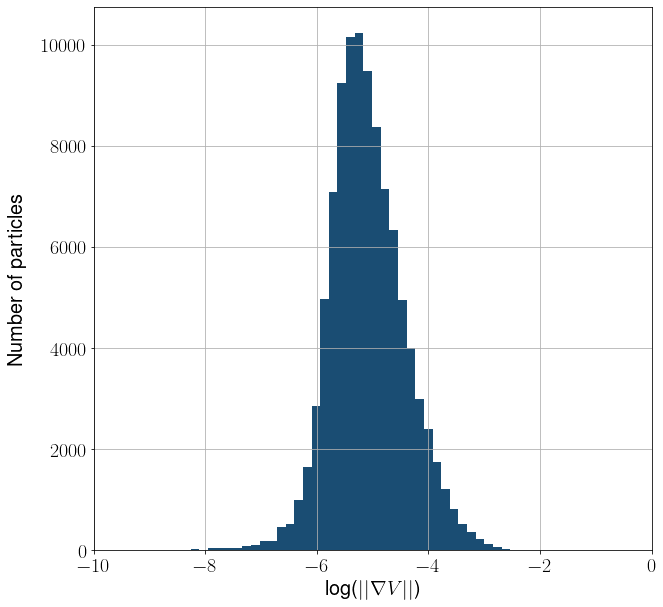
\includegraphics[scale=0.35]{Figures/log_grad_V_hist.png}
			\quad
			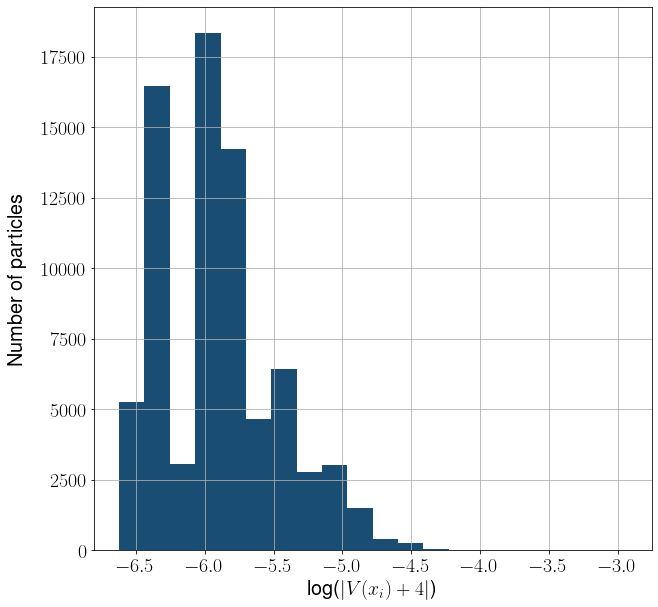
\includegraphics[scale=0.35]{Figures/log_Vp4_hist.png}
			\caption{Left panel: Histogram of the logarithm of the norm of the gradient for each point. Right panel: Histogram of the distance of the value of the potential for each point.}
			\label{fig:Analyze_V_points}
		\end{figure}
		
		The Adam optimizer was employed throughout the gradient descent procedure. It was reinitialized at iterations {250, 500, 750}, with the learning rate fixed at $10^{-2}$. At iteration 1000, the optimizer was reinitialized once more, this time with a reduced learning rate of $10^{-3}$. A final reinitialization was performed at iteration 1500, setting the learning rate to $10^{-4}$, and the optimization was continued for an additional 1000 epochs.
		
		Upon completion, it was observed that all data points converged to values close to $-4$. Specifically, nearly all data points attained values within an absolute error of $10^{-4}$, with the exception of four points whose deviations were on the order of $10^{-3}$. Similarly, 99,739 out of 100,000 data points exhibited gradient norms smaller than $10^{-3}$. These results are summarized in Figure~\ref{fig:Analyze_V_points}.
		
		\begin{figure}
			\centering
			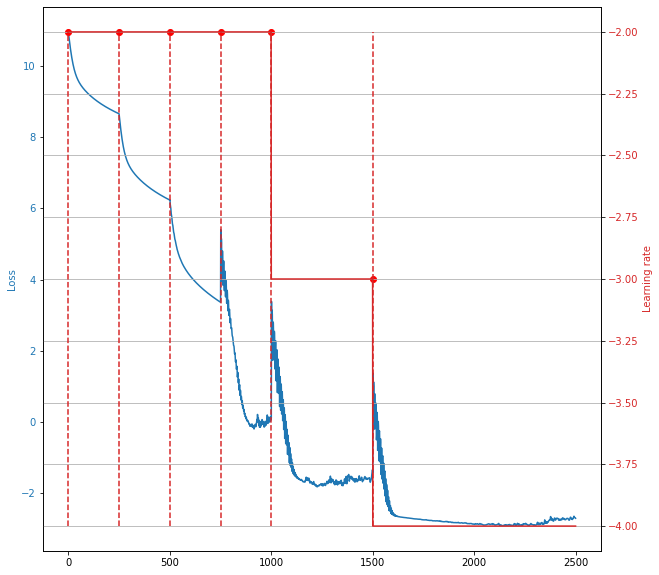
\includegraphics[scale = 0.5]{Figures/Loss_grad_des.png}
			\caption{Evolution of the loss function during gradient descent and corresponding learning rate schedule, noted $\alpha$ on the left y-axis, both plotted on a logarithmic scale. Dashed lines indicate epochs at which the optimizer was reinitialized.}
			\label{fig:loss_grad_des}
		\end{figure}
		
		As a first visualization, we present a triangular plot of the data in Fig. \ref{triangular_plot_1_2_4_8_10}. This figure shows all possible 2D projections of the data, along with the 1D histograms of each coordinate after gradient descent.
		
		\begin{figure}[t]
			\centering
			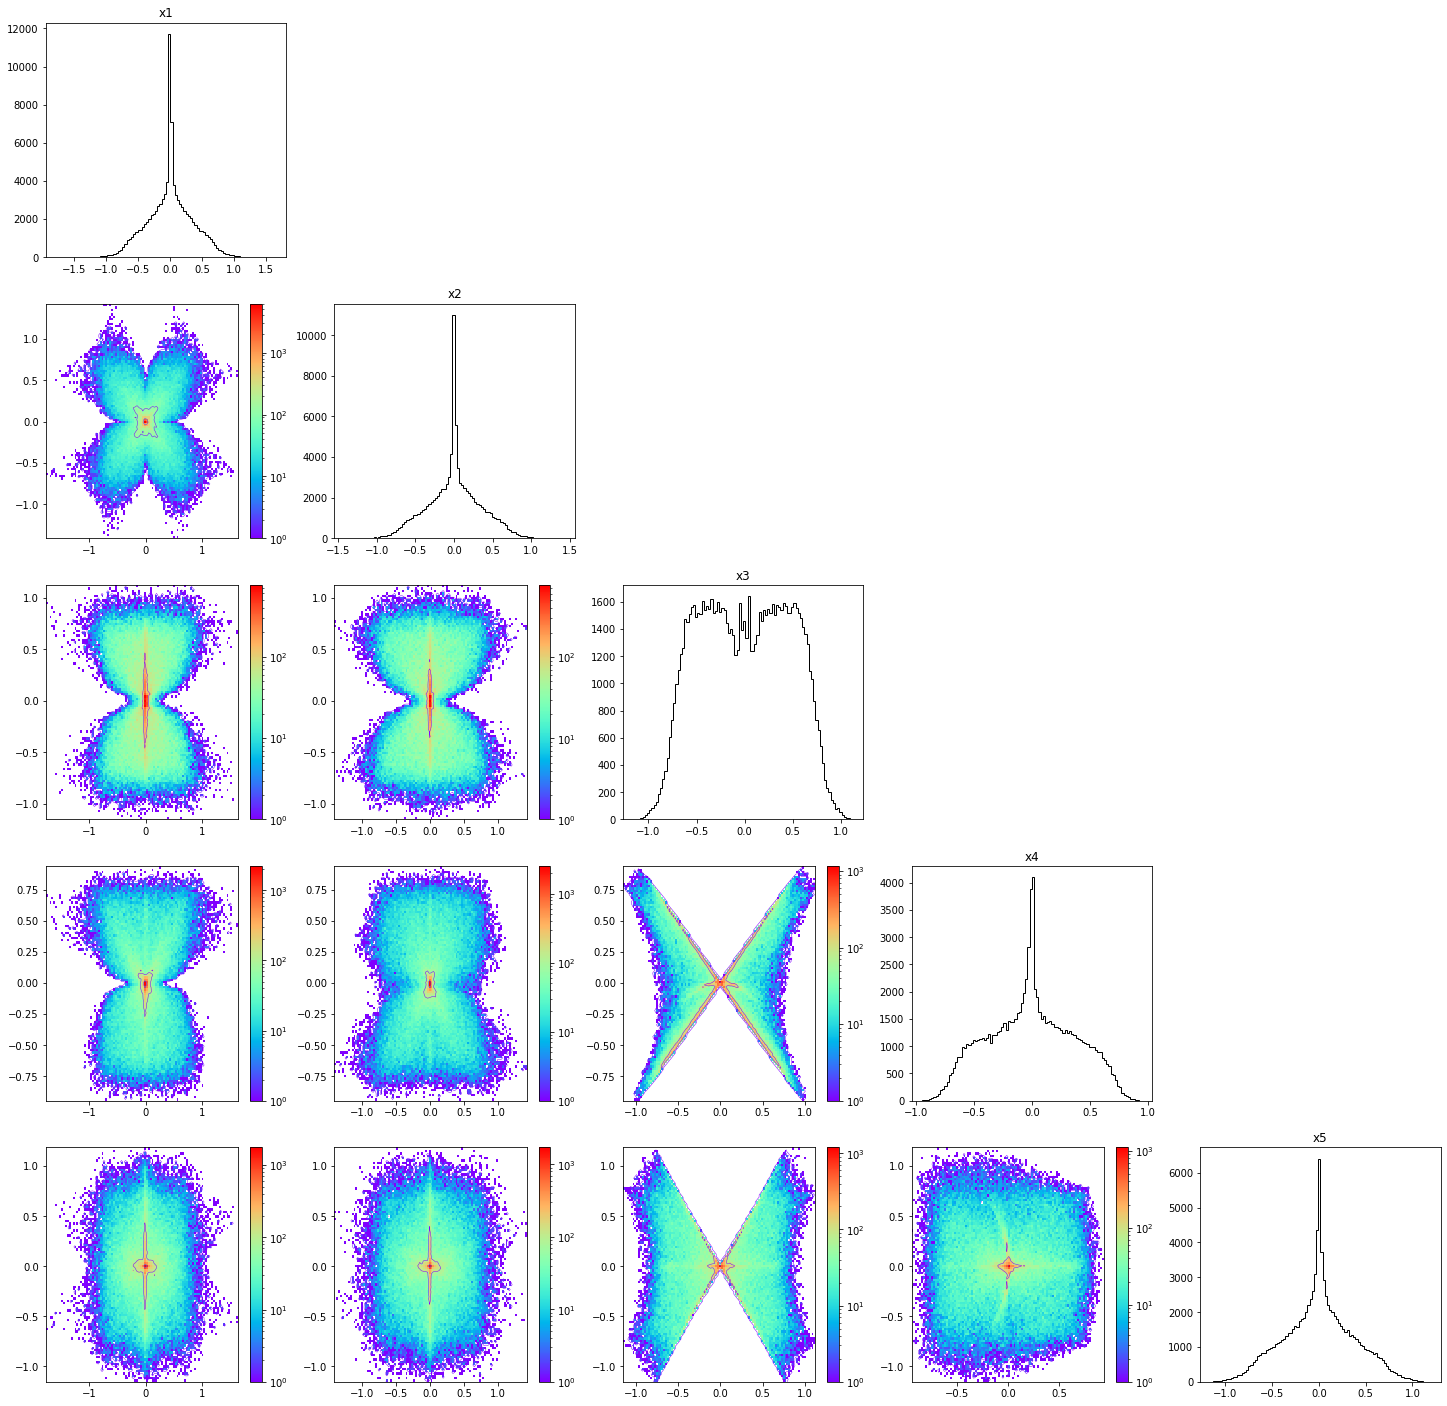
\includegraphics[scale = 0.3]{Figures/triangular_plot_1_2_4_8_10.png} %names need to be changed.
			\caption{Triangular plot showing $2d$ projections and $1d$ histograms of the data after the gradient descent}
			\label{triangular_plot_1_2_4_8_10}
		\end{figure}
		
		We can make a few comments on those plots. First, we observe non-trivial correlations in the data. Some of these may result from larger basins of attraction, such as in the $x_1/x_2$ plot. However, the structures seen in the $x_4/\tilde{x}_8$ or $x_4/x_{10}$ plots likely reflect genuine features of the manifold, and will show latter that this is indeed the case. We also note that all directions appear to be well populated. 
		%Furthermore, we can notice that a large majority of the points converge to the origin $\vec{0}$. This is not surprising, as this just mean that the round sphere solution has a larger basin of attraction, which sounds reasonable. We do not however attempt to shift the points along flat directions to depopulate the origin or repopulate other regions.

		%\paragraph{Local PCA: graphs of number of patches with given local dimension, and with varying size of local patch, discuss optimal patch size (we want at least few points in each direction)}

		Once the gradient descent has been completed and the flat direction sampled, the next step is to identify the structure of the underlying manifold. Our goal is to eventually obtain an analytical expression, not just a numerical description. Before applying symbolic regression to search for such an expression, we can first perform some exploratory analyses to better understand the data. Specifically, we aim to determine the dimensionality of the manifold and wether it consists of a single connected component or multiple disjoint components (e.g., two intersecting hyperplanes).
		
		To this end, we apply a local Principal Component Analysis (PCA). For each point, we identify its $k$ nearest neighbours and perform a PCA on that local neighbourhood. This procedure allows us to determine how many principal directions are needed to explain a given proportion $\epsilon$ of the data variance. In other words, it provides an estimate of the local dimensionality around each point.
		
		We perform this analysis for several values of $k$, namely $k \in \{5, 10, 20, 50, 100\}$, and we fix $\epsilon = 0.99$. The results are presented in Fig. \ref{local_pca}.
		
		\begin{figure}[h!]
			\centering
			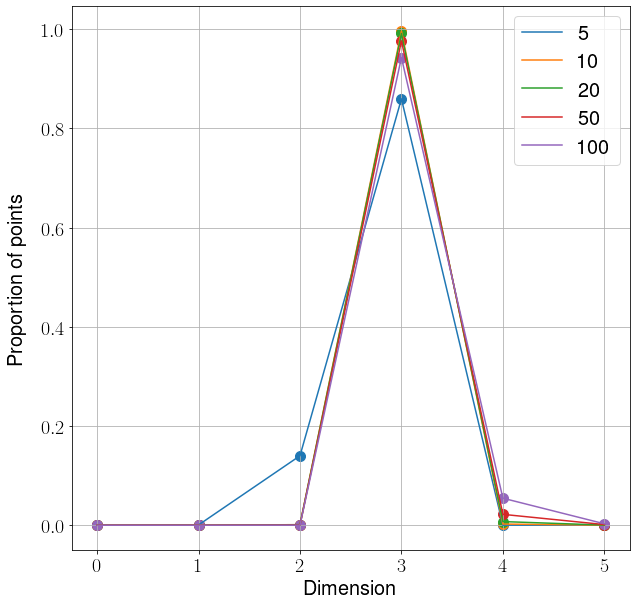
\includegraphics[scale=0.4]{Figures/Local_PCA.png}
			\caption{Results of the local PCA analysis. The $x$-axis shows the dimension inferred by the algorithm, and the $y$-axis indicates the proportion of points for which that dimension was found. Each curve corresponds to a different value of $k$ in the $k$-nearest neighbours.}
			\label{local_pca}
		\end{figure}
		
		We observe that for every choice of $k$, there is a prominent peak at $d = 3$, suggesting that the underlying manifold is three-dimensional. For $k = 5$, a noticeable fraction of points are assigned a dimensionality of 2. This can be attributed to the fact that if the true dimension is 3, then selecting only 5 neighbours may not sufficiently populate all three directions, leading the algorithm to underestimate the dimensionality for a fraction of the points. 
		
		Additionally, for $k \geq 20$, we observe an increasing number of points being assigned dimensionalities of 4 or 5. This behavior can be explained by the loss of locality when the number of neighbours becomes too large: increasing $k$ results in a coarser approximation, and the algorithm may then incorporate points that are no longer truly local. This artificial enlargement of the neighbourhood can cause the estimated local dimensionality to rise.
		
		We thus conclude that the manifold under investigation has an intrinsic dimension of 3.
		
		%\paragraph{Clustering: HDBScan (only parameter: minimal number of points in a cluster), and graphs of 3d slices of the 5d space}
		
		One possible scenario is that our data actually consists of several distinct three-dimensional manifolds, and the points previously identified with dimension $4$ may lie at the intersections of these manifolds. To illustrate, consider the intersection of two lines: at the intersection point, the local dimensionality estimated by the previous PCA algorithm would be 2. To rule out this possibility, we apply a clustering algorithm based on local density, where we only select the points of dimension 3. This, way, we remove the possible intersection points with dimension 4. For the purpose of the clustering, we use the HDBSCAN algorithm\footnote{Details of the algorithm can be found in the original HDBSCAN paper or documentation. Briefly, it is a density-based clustering method that extends DBSCAN by converting it into a hierarchical clustering algorithm and then extracting a flat clustering based on the stability of clusters.}.
		
		We set the minimum cluster size to 10 points. Out of the 98,606 3-dimensional points, the algorithm identifies three clusters: one of size 10, one of size 91,747, and one of size 6,849. 
		
		The smallest cluster (10 points) is likely an artefact of local fluctuations in the data density and is not interpreted as physically meaningful. The last group, comprising 6,849 points, consists of points that the algorithm could not assign to any cluster. We interpret these as outliers or edge points rather than representatives of a separate manifold.
		
		What the algorithm does indicate, however, is that over 90\% of the data belongs to a single dominant cluster. In Fig.~\ref{3dplots}, we show 3D projections of the data to visualize the clustering.
		
		\begin{figure}[h!]
			\centering
			\hspace{-2cm}
			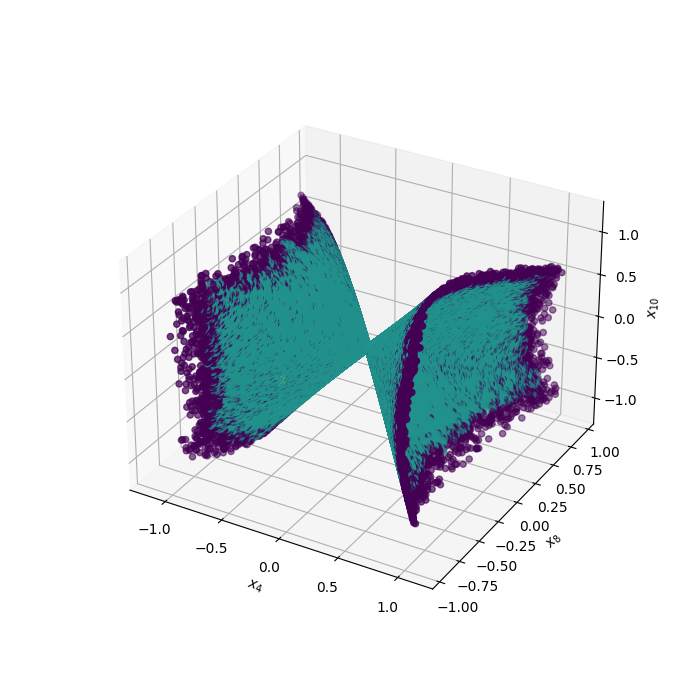
\includegraphics[scale=0.5]{Figures/3d_plot_x4_x8_x10.png}
			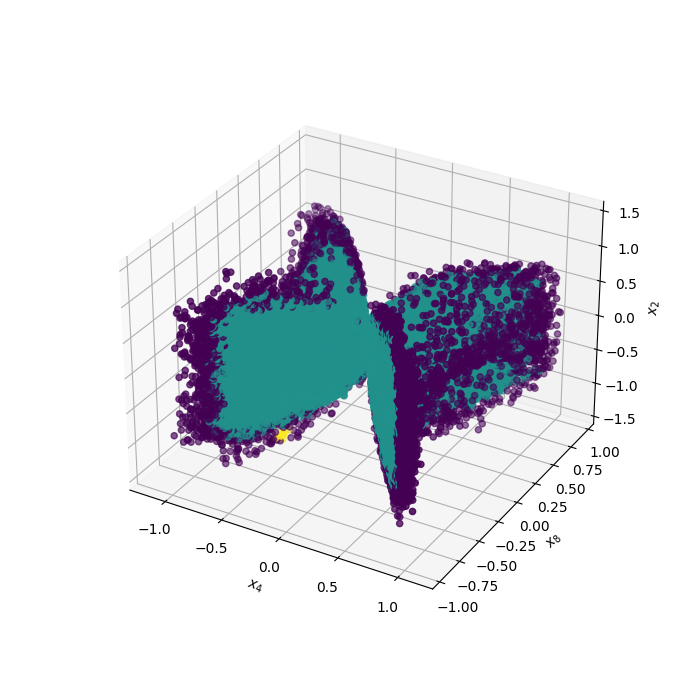
\includegraphics[scale=0.5]{Figures/3d_plot_x2_x4_x8.png}
			\caption{3D plots of the data in selected coordinates. Left: $(x_4, x_8, x_{10})$. Right: $(x_2, x_4, x_8)$.}
			\label{3dplots}
		\end{figure}
		
		In these scatter plots, turquoise points belong to the main cluster, while purple points are those that the algorithm failed to assign. In one of the plots, a few yellow points can be seen; these correspond to the smallest cluster of 10 points. From visual inspection, it appears that the unassigned (purple) points lie mostly on the boundary of the sampled region. We therefore interpret their unassigned status not as evidence of belonging to another manifold, but rather as a result of insufficient local density near the edges of the dataset.
		
		From this analysis, we conclude that the gradient descent procedure has produced a sampling of a single, connected, three-dimensional manifold.
		
		\vspace{0.5em}
		
		After performing both PCA and clustering, we thus confirm that the data obtained after gradient descent samples a three-dimensional manifold.

	\subsection{Annealed Importance Sampling for polynomial symbolic regression}
	%\begin{itemize}[label=\textbullet]
		%\item We can convert the potential to a polynomial by converting the variables that appear in exponentials to logs.
	%\item As the potential is a polynomial, the solutions satisfy polynomials equations. Discuss that fact that we could get polynomials directly by taking the gradient of the potential, but those will be to complicated to express the vacuum in a usable way.  We search those using Annealed Importance Sampling.
		
		Now we have sampled the manifold and extracted some basic information about it (namely its dimension and the fact that it is made of one block), we would like to see if we can extract some analytic formula to characterise it. What we have at the moment, are points on a 3-dimensional manifold, which are embedded in a 5-dimensional space. Therefore we can conclude that, in order to characterise the manifold, we need two independent constraints on the embedding coordinates $\vec{x} = (x_1,x_2,x_4,\tilde{x}_8,x_{10})$. If we have a look at the form of the potential \eqref{eq:scalarpotential124810}, we see that if we use $x_{8} = e^{\tilde{x}_8}$, that, up to a global $e^{-2\tilde{x}_8}$ factor, this potential is actually a polynomial of the embedding coordinates. Therefore, the components of $|\nabla V|$ are also polynomials in those variables. We conclude that the constraints on the embedding coordinates we are looking for are polynomial constraints of the form $p(\vec{x}) = 0$, and that there should be at least two of those. Note that we are now taking $\vec{x} = (x_1,x_2,x_4,\tilde{x}_8,x_{10})$. Of course if one takes directly the gradient of \eqref{eq:scalarpotential124810}, one ends up with such conditions, but none are usable directly to solve for two of the variables in terms of the others. The problem we are facing here is therefore a problem of symbolic regression: we are looking for analytic expressions (polynomial) that vanish once evaluated on our data points. There are a number of way one can deal with it, using already existing methods such as AI Feynman methods~\cite{Udrescu:2019mnk}, or ... \bd{litterature review}. In the spirit of trying to build a generalisable method, we develop here our own method, which is based on symbolic regression using an Annealing Importance Sampling method. 

		%\item Annealed Importance Sampling: first explain general idea (construct density probability, role of temperature, links with Monte-Carlo), discuss $\beta$ to control exploration and exploitation phases.
		
		In the realm of symbolic regression, the aim is to uncover interpretable mathematical expressions that best describe a given dataset. In the problem discussed in this paper, we are looking for polynomial expressions such that $p(\vec{x}^i) = 0$, with $i \in \{1, \dots, \texttt{n\_{sample}}\}$. This task involves navigating a vast, discrete, and often rugged search space of possible symbolic models, which poses significant challenges for traditional sampling methods. Markov Chain Monte Carlo (MCMC) techniques, while widely used, can struggle with poor mixing and getting trapped in local optima, especially in high-dimensional or multimodal spaces.
		
		To address these challenges, we employ an Annealed Importance Sampling (AIS) combined with Sequential Monte Carlo (SMC) methods. AIS constructs a sequence of intermediate distributions that smoothly transition from an initial, tractable distribution (e.g., a prior over symbolic expressions) to the complex target posterior distribution. This annealing process is guided by a temperature-like parameter that gradually emphasizes the data likelihood, allowing for more efficient exploration of the probability landscape.
		
		SMC enhances this procedure by propagating a population of particles—each representing a candidate symbolic expression—through the sequence of distributions. At each step, particles are reweighted based on the incremental change in the distribution, resampled to focus computational effort on high-probability regions, and mutated via operations. This combination of importance sampling, resampling, and mutation maintains diversity among the particles and prevents premature convergence to suboptimal models.
		
		These features make AIS-SMC particularly well-suited for symbolic regression tasks, where the search space is not only high-dimensional but also structured and discontinuous. 
		
		%\item Then more details: discuss hypotheses to compute the weights, choice of transformations, choice of $\beta$, choice of loss, prior, initial sampling, choice of representation for the polynomials.
		
		Let us now explain in more details how does this procedure goes. The goal is to reconstruct some distribution function $d(z)$, where here $z$ in going to be some polynomial. We will try to reconstruct this density function by series of density function $\pi_n(z_n) = \gamma_n(z_n)/Z_n$ with $n = 1,\dots,N$ is going to be the number of annealing steps, $\pi_n$ is defined in terms of an unnormalized density $\gamma_n$ and we have the normalizing constant $Z_n = \int \gamma_n(z) \mathrm{d}z$. We also assume we have a sequence of inverse temperature constants $\beta_n$, where $0 = \beta_1 < \beta_2 <\dots< \beta_N = 1$. We then define the unnormalized density at level $n$ in terms of a prior distribution $p_0(z)$ over the hypothesis space and a loss function $L(z)$:
		\begin{equation}
			\gamma_n(z) := d_0(z) \: \exp \left( -\beta_n L(z) \right).
		\end{equation} 
		
		At each step, we have a set of particles and weights $\{z_{n-1}^k, w_{n-1}^k\}$ approximating $\pi_{n-1}$ (meaning $\mathbb{E}_{\pi_{n-1}}[f] \approx \frac{\sum_k w_{n-1}^k f(z_{n-1}^k)}{\sum_k w_{n-1}^k}$), and we want to obtain a new set $\{z_n^k, w_n^k\}$ approximating $\pi_n$. To do so, for each particle $z^k_{n-1}$, we propose a new particle $z_n^k \sim q(z_n | z_{n-1}^k)$ and calculate the new unnormalized importance weight $w_n^k$. The latter are updated using the formula 
		\begin{equation}
			w_n^k = w_{n-1}^k \times \alpha_{n}^k
		\end{equation}
		where $\alpha_n^k$ is the incremental importance weight. The standard form for $\alpha_n^k$, which requires introducing an auxiliary backward transition kernel $q(z_{n-1} | z_n)$, is:
		\begin{equation}
			\alpha_n^k = \frac{ \gamma_n(z_n^k) q(z_{n-1}^k | z_n^k) }{ \gamma_{n-1}(z_{n-1}^k) q(z_n^k | z_{n-1}^k) } 
		\end{equation}
		The weights are finally normalized and we get $w_n^k \rightarrow \frac{w_n^k}{\sum_j w_n^j}$.
		
		Let's us now focus on the forward $q(z_n^k | z_{n-1}^k)$ and backward propagation kernel $q(z_{n-1}^k | z_n^k)$ for now. The forward propagation kernel defines how we generate the state at time $n$ given the state at time $n-1$. It gives the probability to transition from $z_{n-1}$ to $z_n$. The backward kerne represents a hypothetical probability of transitioning back from state $z_n$ to state $z_{n-1}$. The purpose of $q$ is to give a proposition for $z_n$ given $z_{n-1}$. For the implementation of the two, we decide to implement an AIS-style MCMC code : we make some move in the space of polynomials, and then accept or reject those new polynomials based on an acceptance rate. So we first need to choose what are the available moves in the space of polynomials. Here are the choices we have made for our symbolic regression task : 
		\begin{itemize}
			\item Coefficient pertubation. Given a polynomial $z_{n-1}$, we choose randomly one of his coefficient and modify it by a random noise from the guassian distribution $\mathcal{N}(0,\sigma^2)$. So for eg : $2 x_1 + 3 x_2^2 \rightarrow  2.1 x_1 + 3 x_2^2$.
			\item Variable multiplication. Given a polynomial $z_{n-1}$, we choose randomly one of his monomial, and multiply it by one of the available variable. So for eg : $2 ^x_1 + 3 x_2^2 \rightarrow  2 x_1 x_2 + 3 x_2^2$.
			\item Variable division. Given a polynomial $z_{n-1}$, we choose randomly one of his monomial, and divide it by one of its variable. So for eg : $2 x_1 + 3 x_2^2 \rightarrow  2 x_1 x_2 + 3 x_2^2$. 
		\end{itemize}
		This implementation enables a direct computation of both the forward and backward propagation kernels. In particular, for the case of coefficient perturbations, the transition is symmetric. That is,
		\begin{equation}
			q(z_n^k \mid z_{n-1}^k) = q(z_{n-1}^k \mid z_n^k),
		\end{equation}
		which significantly simplifies the computation of the incremental importance weight.
		
		However, this symmetry does not hold in general. For other types of operations—such as multiplication or division by a variable—the transition from \( z_{n-1}^k \) to \( z_n^k \) is generally not equivalent to the reverse transition from \( z_n^k \) to \( z_{n-1}^k \). In such cases $q(z_n^k \mid z_{n-1}^k) \ne q(z_{n-1}^k \mid z_n^k)$ and particular care must be taken in the computation of the backward propagation kernel.
		
		
		The acceptance ratio for the MCMC algorithm is given by : 
		\begin{equation}
			A(z_n,z_{n-1}) = \mathrm{min} \left(1,\frac{ \gamma_n(z_n^k) q(z_{n-1}^k | z_n^k) }{ \gamma_{n-1}(z_{n-1}^k) q(z_n^k | z_{n-1}^k) }  \right)
		\end{equation}
		We then draw $u\sim \mathrm{Uniform}(0,1)$, accept the new particle if $u<A(z_n,z_{n-1})$ and reject it otherwise.
		
		Before closing the section, we need to discuss what is the Loss function we choose. It is required to compute the unormalized distribution $\gamma_n$. Assume that we have $z = \sum_k c_k X_k$, where $c_k$ are the coefficients of the polynomials, and $X_k$ is a short notations for all the possible monomials up to a given degree (so if we have $x$ and $y$ as variables, and the maximum degree is 2, then $X_k$ are $1, x, y, x^2, y^2, x y$). For the Loss function, we decided to take : 
		\begin{equation}
			L(z) = \sum_{i} z(x_i)^2 + \frac{\lambda}{\sum_k c_k}
		\end{equation}
		So the first term is just the sum of the squared of the polynomial evaluated on the data. We want to make this 0 so we find polynomial that annihilates our data. The second part is a regularisation factor : it prevents the algorithm to send all the coefficient to 0, which would give a trivial solution to the problem. We typically take $\lambda \sim \mathcal{O}(1000)$.
		
		%\item Analysis after AIS: select the best polynomials and do exploitation on the coefficients (without MC: we keep only the proposal of it betters the polynomial).
		
		Once the Annealing loop is over, we end up with a total of $n_{sample}$ particles, which in principle should be close to annihilate our data, but whose coefficient may need some more fine tuning. To deal with it, we ran a quick exploitation phase, where, for each polynomial, we now only modify its coefficients, with a pertubation $\epsilon \sim \mathcal{N}(0, \sigma_1)$, and keep the new particle, only if the Loss function is now getting smaller. This allow to fine-tune the coefficients. 
		
		\bd{Results for naive choices of parameters (numbers of iteration and particles, probabilities, $\beta$) and motivate them (we want some exploration and then exploitation, not too long computations): for multiple runs we find multiple polynomials (good polynomial: after exploitation we convert the coefficients to integers and square roots, and recompute loss without regularisation, select with threshold). Quantify it nicely: success rates for each polynomials, and absolute number of success, failing rate. Total time needed, without cluster or fancy computers.}
	%\end{itemize}
	
	\paragraph{Results}
	We have used the numerical analysis outlined in the previous sections to the search for extrema of the scalar potential~\eqref{eq:scalarpotential}. The code finds the 8 different following polynomials: 
	\begin{subequations} \label{eq:pols}
    \begin{align}
      p_{1} &= -\sqrt{2}\,x_{1} + \sqrt{2}\,x_{1}x_8 + x_{2}x_8x_{10} - \sqrt{2}\,x_{2}x_{4}x_8,\\
      p_{2} &= 2\,x_{2} - 2\,x_{2}x_8 + \sqrt{2}\,x_{1}x_{10} + 2\,x_{1}x_{4} - x_{2}x_8x_{10}^{2},\\
      p_{3} &= 2\,x_{2} - 2\,x_{2}x_8 + \sqrt{2}\,x_{1}x_8x_{10} + 2\,x_{1}x_{4}x_8
      		- 2\,x_{2} x_{4}^{2}x_8,\\
      p_{4} &= \sqrt{2}\,x_{2} - \sqrt{2}\,x_{2}x_8 + \sqrt{2}\,x_{1}\,x_{4} + x_{1}x_8x_{10}
      		- x_{2}x_{4}x_8x_{10},\\
      p_{5} &= -2\,x_{1} - 2\,x_{2}x_{4}- 2\,x_{1}x_{4}^{2} + 2\,x_{1}x_8 + \sqrt{2}\,x_{2}x_{10}
      		+ x_{1}x_8x_{10}^{2},\\
      p_{6} &= -2\,x_{2}x_{4} - 2\,x_{1}x_{4}^{2} + 2\,x_{2}x_{4}x_8 + \sqrt{2}\,x_{2}x_{10} 
      		- \sqrt{2}\,x_{2}x_8x_{10} +  x_{1}x_8x_{10}^{2},\\
      p_{7} &= -\sqrt{2}\,x_{1}^{2}x_{4} + \sqrt{2}\,x_{2}^{2}x_{4} + \sqrt{2}\,x_{1}x_{2}x_{4}^{2} - x_{1}^{2}x_{10}
      		- x_{2}^{2}x_{10}, \\
      p_{8} &= -2 + 4 x_{8} - 2 x_8^2 + 2 x_{4}^2 x_8 - x_8^2 x_{10}^2
    \end{align}
  \end{subequations}
  where $x_{8} = e^{\tilde{x}_{8}}$. They are found with different frequencies, depending on the chosen parameters.
  
  	Let us clarify a point regarding the expected structure of the solutions to the system defined by the critical points of the scalar potential, i.e., the variety defined by the vanishing of the gradient $\nabla V$.
  
  In algebraic geometry, the set of solutions to the equations $\nabla V = 0$ defines an algebraic variety over a certain base field. In our case, the potential $V$ and its gradient $\nabla V$ are polynomial functions with coefficients lying in a specific field extension of $\mathbb{Q}$—typically of the form $\mathbb{Q}(\sqrt{d_1}, \sqrt{d_2}, \dots)$, where $d_i \in \mathbb{Q}$. That is, the coefficients of the polynomials are combinations of rational numbers and square roots of rational numbers.
  
  The conformal manifold (or the moduli space of solutions) is then a subvariety of this ambient space, defined as the common zero locus of the polynomials in $\nabla V$. From the perspective of algebraic geometry, this variety is cut out by an ideal in the polynomial ring with coefficients in the aforementioned field extension of $\mathbb{Q}$. Since the defining equations have coefficients in this field, the variety itself is defined over that same field.
  
  Now, consider the numerical solutions obtained via methods such as annealed importance sampling. If these numerical procedures converge to points on the same variety, and assuming that the variety is irreducible over the given field, then any point (i.e., any solution) on the variety must lie in the same field extension over which the variety is defined. This follows from basic principles in algebraic geometry: the set of algebraic points on a variety defined over a field $K$ are themselves algebraic over $K$, and the field of definition of these points must be a (possibly finite) extension of $K$.
  
  Therefore, even if the numerical solver does not explicitly reveal this, one should expect that the coordinates of the solutions (i.e., the values of the scalar fields at critical points) lie in the same field extension of $\mathbb{Q}$ as the coefficients of the original system of polynomials $\nabla V$. That is, they should belong to $\mathbb{Q}(\sqrt{d_1}, \sqrt{d_2}, \dots)$ or a finite extension thereof.
  
  This argument justifies the expectation that if the scalar potential $V$ and its gradient $\nabla V$ involve only rational numbers and square roots, then the solutions to $\nabla V = 0$—regardless of how they are found—should also lie within the same field extension.
  
  This is this argument that allowed us to round the coefficients of the polynomials given by the annealed importance sampling algorithm, and found the polynomials in \ref{eq:pols}.

  \begin{enumerate}
  		\item {\bfseries \boldmath $\beta$ in power $3$, $\sigma = 0.1$, $\texttt{sample\_size} = 10000$}

	  For 100 runs with parameters
		\begin{equation} \label{eq:sample10000beta3}
			\begin{gathered}
				\texttt{max degree} = 4, \quad \texttt{max num monomials} = 6, \quad n_{\rm iter} = 1000, \quad n_{\rm particles} = 1000, \\
				\texttt{sample size} = 10000, \quad {\rm reg} = 10^{3}, \quad \beta = 10^{-10} + \left(\frac{i}{n_{\rm iter}}\right)^{3}, \quad \sigma = 0.1, \\
				p_{\rm add} = 0, \quad p_{\rm remove} = 0, \quad p_{\rm modify} = 0.5, \quad p_{\rm multiply} = 0.25, \quad p_{\rm divide} = 0.25,
			\end{gathered}
		\end{equation}
		the polynomials are found at the following frequencies
	  \begin{equation}
	  	\begin{tabular}{l|cccccccc}
	  		& $p_{1}$ & $p_{2}$ & $p_{3}$ & $p_{4}$ & $p_{5}$ & $p_{6}$ & $p_{7}$ & $\varnothing$ \\\hline\hline
	  		Frequency & 76\% & 18\% & 10\% & 6\% & 4\% & 1\% & 2\% & 6\%
	  	\end{tabular}
	  \end{equation}
	  The dynamics of the appearance of the target polynomials is plotted in fig.~\ref{fig:sample10000beta3}.

	  Averaged number of particles reproducing a target in a successful run: $973 \pm 103$

	  Mean loss with regularisation for particles reproducing a target: $854 \pm 427$

	  Mean loss without regularisation for particles reproducing a target: $602 \pm 417$

	  \begin{figure}[h!]
	  	\centering
	  	\begin{tikzpicture}
	  		\draw (0,0) node (fig1) {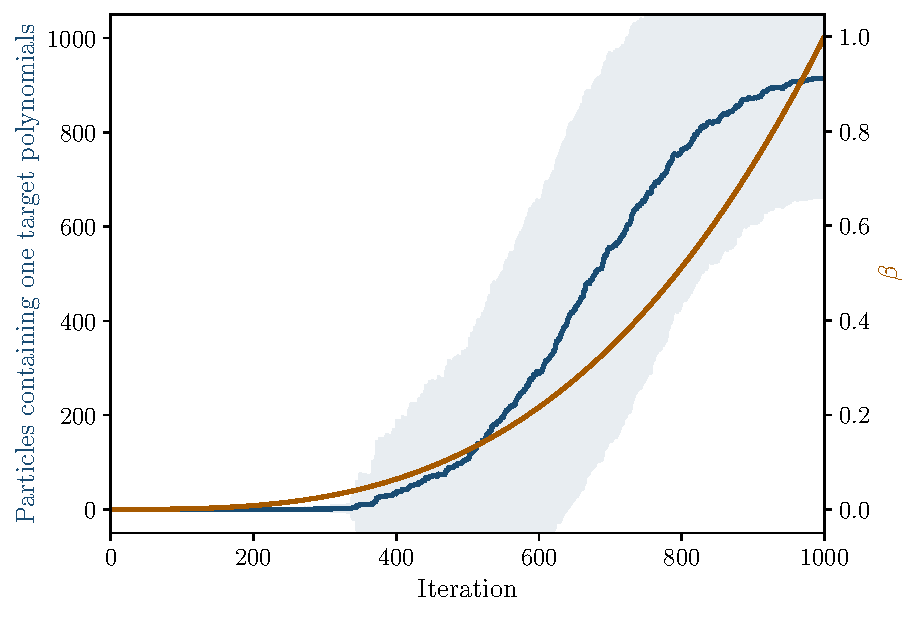
\includegraphics[scale=0.75]{Figures/Count_beta_history_2025_05_19_at_06_01_21.pdf}};
	  		\draw ($(fig1.north west) + (0,0)$) node {\small (a)};
	  		\draw (0,-8) node (fig2) {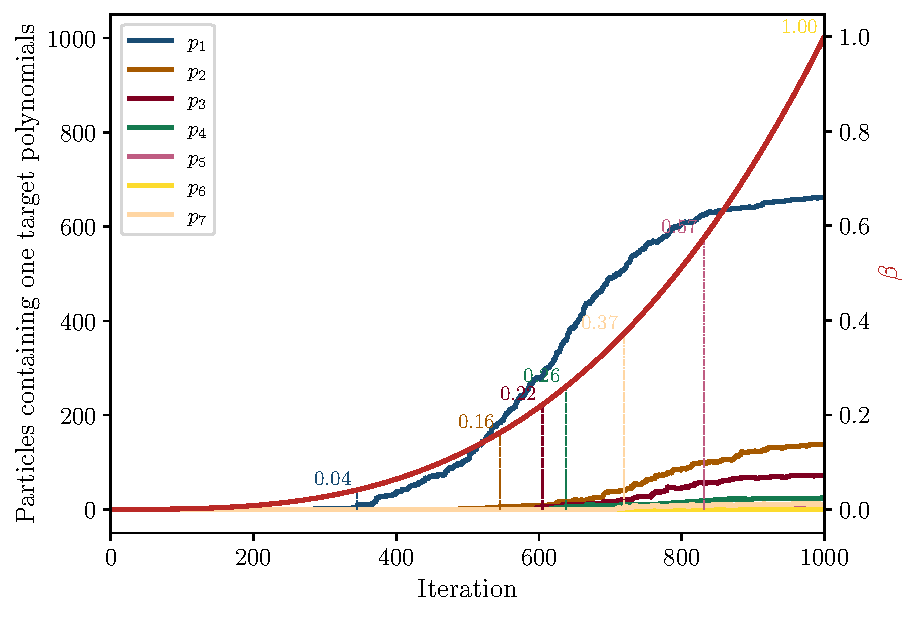
\includegraphics[scale=0.75]{Figures/Count_beta_history_2025_05_19_at_06_01_21_detailed.pdf}};
	  		\draw ($(fig2.north west) + (0,0)$) node {\small (b)};
	  	\end{tikzpicture}
	  	\caption{{\bfseries \boldmath $\beta$ in power $3$, $\sigma = 0.1$, $\texttt{sample size} = 10000$} (a) Evolution of the mean numbers of particles reproducing a target polynomials and its $1\sigma$ deviation for the parameters~\eqref{eq:sample10000beta3}. (b) Evolution of the mean numbers of particles reproducing each targets polynomial. The vertical lines indicate when there are an average 5 particles reproducing a given polynomial, and the value of $\beta$ at that moment.}
	  	\label{fig:sample10000beta3}
	  \end{figure}

	  After the AIS, we performed an exploitation phase to fine tune the coefficients. The distributions of the particles with respect to their loss (without regularisation), is plotted in fig.~\ref{fig:distlocalsearch}. The fine tuning (with \texttt{local\_search}) is made using the loss with regularisation.

	  \begin{figure}[h!]
	  	\centering
	  	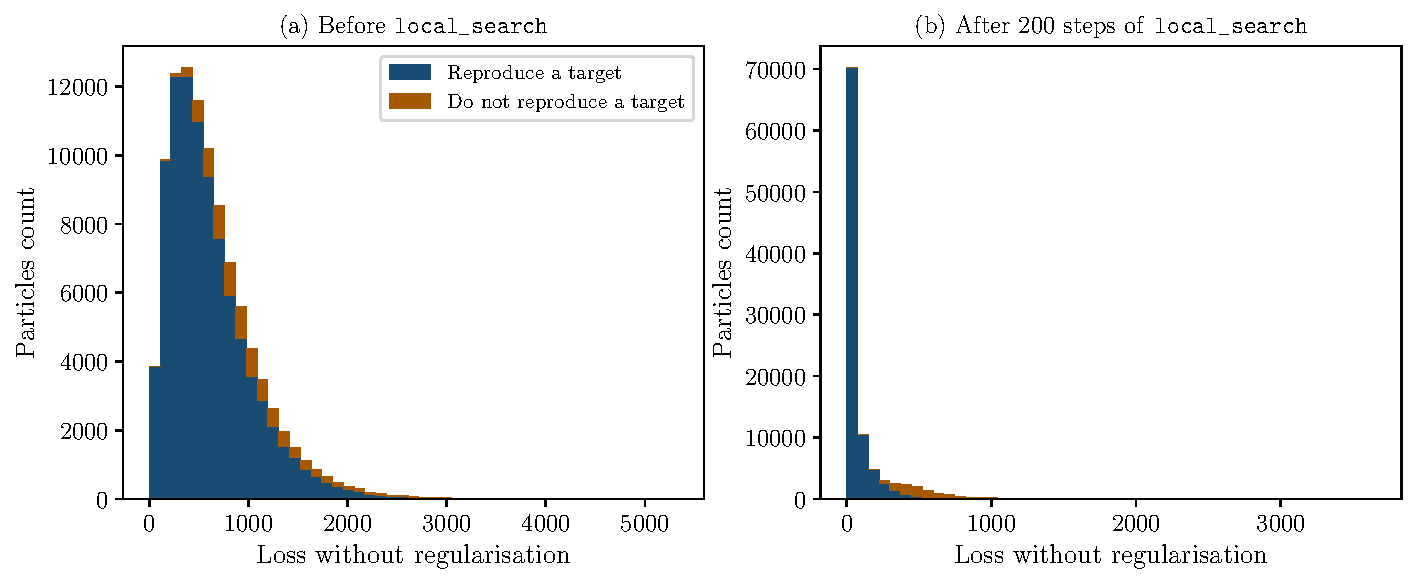
\includegraphics[scale=0.75]{Figures/Local_search_2025_05_19_at_06_01_21.pdf}
	  	\caption{{\bfseries \boldmath $\beta$ in power $3$, $\sigma = 0.1$, $\texttt{sample size} = 10000$} Distributions of all the 100,000 particles with respect to their loss (without regularisation) (a) directly after AIS with parameters~\eqref{eq:sample10000beta3} and (b) after 200 steps of \texttt{local\_search}. The fine tuning (with \texttt{local\_search}) is made using the loss with regularisation.}
	  	\label{fig:distlocalsearch}
	  \end{figure}

	  We list below, for each polynomials in eq.~\eqref{eq:pols}, one example of representing particles directly after AIS and after the fine tuning, and the associated losses (without regularisation):
	  \begin{align}
	  	p_{1}:&\quad
	  	\begin{aligned}
	  		&-1.939\,x_{1} + 2.120\,x_{1}\tilde{x}_{8} + x_{10}x_{2}\tilde{x}_{8} - 2.266\, x_{2}x_{4}\tilde{x}_{8} + 0.029\,x_{2}^{2}x_{4},\quad L^{(\lambda = 0)} \simeq 754, \\
			&-1.416\,x_{1} + 1.414\, x_{1}\tilde{x}_{8} + x_{10}x_{2}\tilde{x}_{8} - 1.414\,x_{2}x_{4}\tilde{x}_{8} + 0.00001\,x_{2}^{2}x_{4},\quad L^{(\lambda = 0)} \simeq 0.0040,
	  	\end{aligned} \\[7pt]
	  	p_{2}:&\quad
	  	\begin{aligned}
	  		&2.213\,x_{2} - 2.075\,x_{2}\tilde{x}_{8} + 1.674\,x_{1}x_{10} + 2.015\,x_{1}x_{4} - x_{10}^{2}x_{2}\tilde{x}_{8},\quad L^{(\lambda = 0)} \simeq 244, \\
			&2.002\,x_{2} - 2.002\,x_{2}\tilde{x}_{8} + 1.417\,x_{1}x_{10} + 2.001\,x_{1}x_{4} - x_{10}^{2}x_{2}\tilde{x}_{8},\quad L^{(\lambda = 0)} \simeq 0.015,
	  	\end{aligned} \\[7pt]
	  	p_{3}:&\quad
	  	\begin{aligned}
	  		&2\,x_{2} - 1.808\,x_{2}\tilde{x}_{8} + 1.168\,x_{1}\tilde{x}_{8}x_{10} + 1.828\,x_{1}x_{4}\tilde{x}_{8} - 1.864\,x_{2}x_{4}^{2}\tilde{x}_{8},\quad L^{(\lambda = 0)} \simeq 180, \\
			&2\,x_{2} - 1.998\,x_{2}\tilde{x}_{8} + 1.412\,x_{1}\tilde{x}_{8}x_{10} + 1.998\,x_{1}x_{4}\tilde{x}_{8} - 1.998\,x_{2}x_{4}^{2}\tilde{x}_{8},\quad L^{(\lambda = 0)} \simeq 0.016,
	  	\end{aligned} \\[7pt]
	  	p_{4}:&\quad
	  	\begin{aligned}
	  		&1.458\,x_{2} - 1.341\,x_{2}\tilde{x}_{8} + 1.497\,x_{1}x_{4} + x_{1}\tilde{x}_{8}x_{10} - 1.008\,x_{2}x_{4}\tilde{x}_{8}x_{10} + 0.020 x_{2}^{2}x_{4}\tilde{x}_{8},\quad L^{(\lambda = 0)} \simeq 218, \\
			&1.419\,x_{2} - 1.418\,x_{2}\tilde{x}_{8} + 1.416\,x_{1}x_{4} + x_{1}\tilde{x}_{8}x_{10} - 1.001\,x_{2}x_{4}\tilde{x}_{8}x_{10} - 0.0003\,x_{2}^{2}x_{4}\tilde{x}_{8},\quad L^{(\lambda = 0)} \simeq 0.074,
	  	\end{aligned} \\[7pt]
	  	p_{5}:&\quad
	  	\begin{aligned}
	  		&-2.179\,x_{1} - 1.571\,x_{2}x_{4} - 1.953\,x_{1}x_{4}^{2} + 1.983\,x_{1}\tilde{x}_{8} + 1.530\,x_{2}x_{10} + x_{1}\tilde{x}_{8}x_{10}^{2},\quad L^{(\lambda = 0)} \simeq 210, \\
			&-2.008\,x_{1} - 2.001\,x_{2}x_{4} - 1.999\,x_{1}x_{4}^{2} + 1.995\,x_{1}\tilde{x}_{8} + 1.412\,x_{2}x_{10} + x_{1}\tilde{x}_{8}x_{10}^{2},\quad L^{(\lambda = 0)} \simeq 0.228,
	  	\end{aligned} \\[7pt]
	  	p_{6}:&\quad
	  	\begin{aligned}
	  		&- 2.856\,x_{2}x_{4} - 2.499\,x_{1}x_{4}^{2} + 2.721\,x_{2}x_{4}\tilde{x}_{8} + 1.677\,x_{2}x_{10} - 1.187\,x_{2}\tilde{x}_{8}x_{10} + x_{1}\tilde{x}_{8}x_{10}^{2} ,\quad L^{(\lambda = 0)} \simeq 202, \\
			&- 2.043\,x_{2}x_{4} - 2.005\,x_{1}x_{4}^{2} + 2.030\,x_{2}x_{4} \tilde{x}_{8} + 1.393\,x_{2}x_{10} - 1.401\,x_{2}\tilde{x}_{8}x_{10} + x_{1}\tilde{x}_{8}x_{10}^2 ,\quad L^{(\lambda = 0)} \simeq 1.28,
	  	\end{aligned} \\[7pt]
	  	p_{7}:&\quad
	  	\begin{aligned}
	  		&- 1.354\,x_{1}^{2}x_{4} + 1.243\,x_{2}^{2}x_{4} + 1.304\,x_{1}x_{2}x_{4}^{2} - 1.053\,x_{1}^{2}x_{10} - x_{2}^{2}x_{10} + 0.052\,x_{2}x_{4}^{2}x_{10} ,\quad L^{(\lambda = 0)} \simeq 373, \\
			&- 1.413\,x_{1}^{2}x_{4} + 1.415\,x_{2}^{2}x_{4} + 1.413\,x_{1}x_{2}x_{4}^{2} - 0.997\,x_{1}^{2}x_{10} - x_{2}^{2}x_{10} + 0.0003\,x_{2}x_{4}^{2}x_{10} ,\quad L^{(\lambda = 0)} \simeq 0.038.
	  	\end{aligned}
	  \end{align}

	  \item {\bfseries \boldmath $\beta$ in power $4$, $\sigma = 0.1$, $\texttt{sample size} = 10000$}

	  For 100 runs with parameters
		\begin{equation} \label{eq:sample10000beta4}
			\begin{gathered}
				\texttt{max degree} = 4, \quad \texttt{max num monomials} = 6, \quad n_{\rm iter} = 1000, \quad n_{\rm particles} = 1000, \\
				\texttt{sample size} = 10000, \quad {\rm reg} = 10^{3}, \quad \beta = 10^{-10} + \left(\frac{i}{n_{\rm iter}}\right)^{4}, \quad \sigma = 0.1, \\
				p_{\rm add} = 0, \quad p_{\rm remove} = 0, \quad p_{\rm modify} = 0.5, \quad p_{\rm multiply} = 0.25, \quad p_{\rm divide} = 0.25,
			\end{gathered}
		\end{equation}
		the polynomials are found at the following frequencies
	  \begin{equation}
	  	\begin{tabular}{l|cccccccc}
	  		& $p_{1}$ & $p_{2}$ & $p_{3}$ & $p_{4}$ & $p_{5}$ & $p_{6}$ & $p_{7}$ & $\varnothing$ \\\hline\hline
	  		Frequency & 74\% & 17\% & 7\% & 8\% & 2\% & 0\% & 2\% & 6\%
	  	\end{tabular}
	  \end{equation}
	  The dynamics of the appearance of the target polynomials is plotted in fig.~\ref{fig:sample10000beta4}.

	  Averaged number of particles reproducing a target in a successful run: $951 \pm 200$

	  Mean loss with regularisation for particles reproducing a target: $709 \pm 320$

	  Mean loss without regularisation for particles reproducing a target: $452 \pm 309$

	  \begin{figure}[h!]
	  	\centering
	  	\begin{tikzpicture}
	  		\draw (0,0) node (fig1) {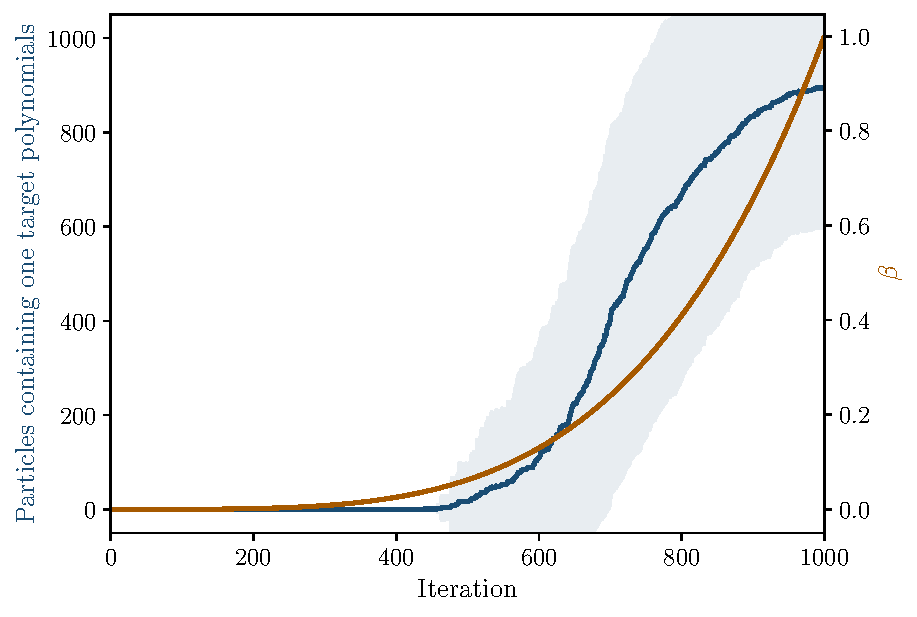
\includegraphics[scale=0.75]{Figures/Count_beta_history_2025_05_22_at_08_48_38.pdf}};
	  		\draw ($(fig1.north west) + (0,0)$) node {\small (a)};
	  		\draw (0,-8) node (fig2) {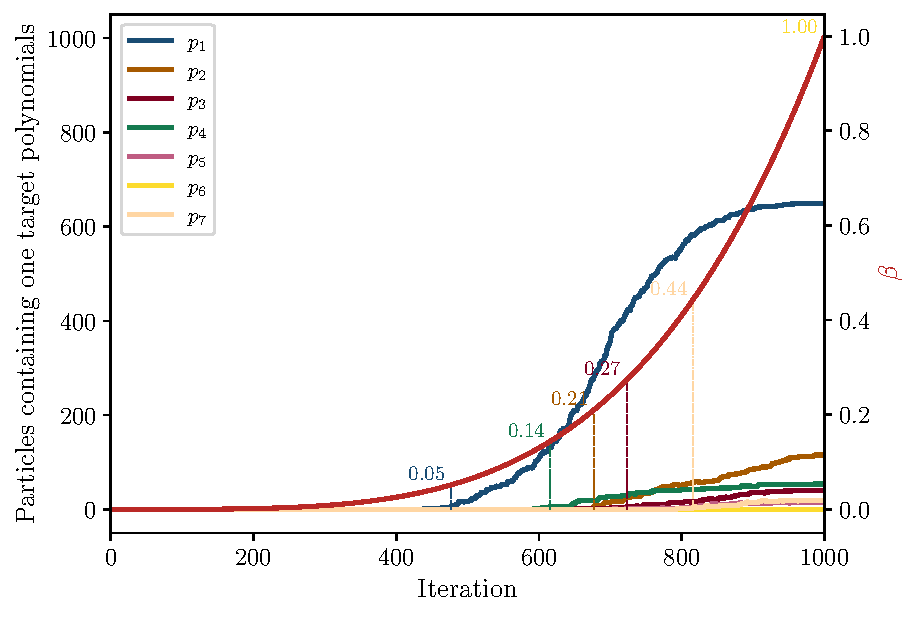
\includegraphics[scale=0.75]{Figures/Count_beta_history_2025_05_22_at_08_48_38_detailed.pdf}};
	  		\draw ($(fig2.north west) + (0,0)$) node {\small (b)};
	  	\end{tikzpicture}
	  	\caption{{\bfseries \boldmath $\beta$ in power $4$, $\sigma = 0.1$, $\texttt{sample size} = 10000$} (a) Evolution of the mean numbers of particles reproducing a target polynomials and its $1\sigma$ deviation for the parameters~\eqref{eq:sample10000beta4}. (b) Evolution of the mean numbers of particles reproducing each targets polynomial. The vertical lines indicate when there are an average 5 particles reproducing a given polynomial, and the value of $\beta$ at that moment.}
	  	\label{fig:sample10000beta4}
	  \end{figure}

	  \item {\bfseries \boldmath $\beta$ in power $5$, $\sigma = 0.1$, $\texttt{sample size} = 10000$}

  		For 100 runs with parameters
		\begin{equation}
			\begin{gathered}
				\texttt{max degree} = 4, \quad \texttt{max num monomials} = 6, \quad n_{\rm iter} = 1000, \quad n_{\rm particles} = 1000, \\
				\texttt{sample size} = 10000, \quad {\rm reg} = 10^{3}, \quad \beta = 10^{-10} + \left(\frac{i}{n_{\rm iter}}\right)^{5}, \quad \sigma = 0.1, \\
				p_{\rm add} = 0, \quad p_{\rm remove} = 0, \quad p_{\rm modify} = 0.5, \quad p_{\rm multiply} = 0.25, \quad p_{\rm divide} = 0.25,
			\end{gathered}
		\end{equation}
		the polynomials are found at the following frequencies
	  \begin{equation}
	  	\begin{tabular}{l|cccccccc}
	  		& $p_{1}$ & $p_{2}$ & $p_{3}$ & $p_{4}$ & $p_{5}$ & $p_{6}$ & $p_{7}$ & $\varnothing$ \\\hline\hline
	  		Frequency & 69\% & 11\% & 7\% & 12\% & 0\% & 4\% & 0\% & 13\%
	  	\end{tabular}
	  \end{equation}
	  The dynamics of the appearance of the target polynomials is plotted in fig.~\ref{fig:sample10000beta5}.

	  Averaged number of particles reproducing a target in a successful run: $960 \pm 175$

	  Mean loss with regularisation for particles reproducing a target: $606 \pm 257$

	  Mean loss without regularisation for particles reproducing a target: $359 \pm 244$

	  \begin{figure}[h!]
	  	\centering
	  	\begin{tikzpicture}
	  		\draw (0,0) node (fig1) {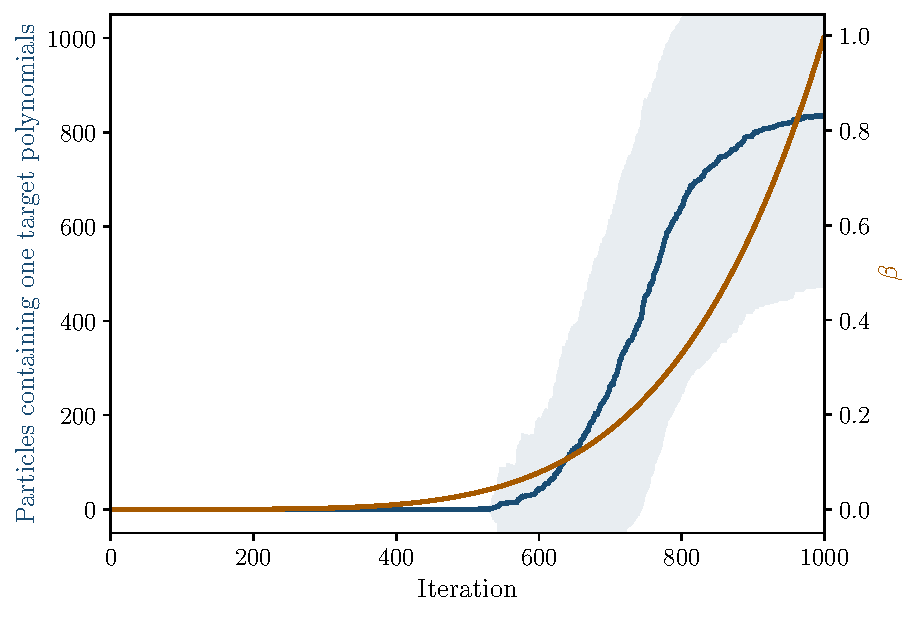
\includegraphics[scale=0.75]{Figures/Count_beta_history_2025_05_18_at_06_28_32.pdf}};
	  		\draw ($(fig1.north west) + (0,0)$) node {\small (a)};
	  		\draw (0,-8) node (fig2) {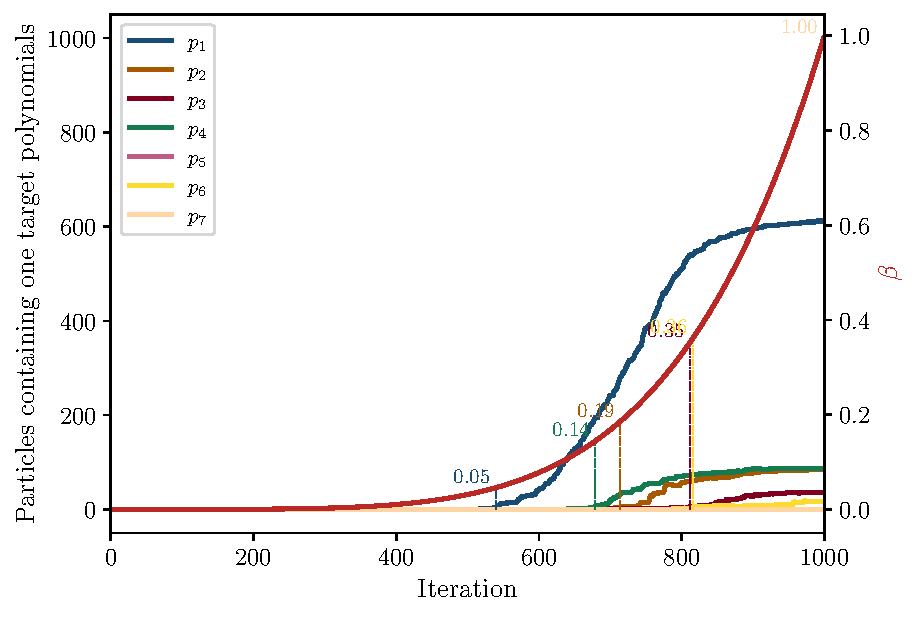
\includegraphics[scale=0.75]{Figures/Count_beta_history_2025_05_18_at_06_28_32_detailed.pdf}};
	  		\draw ($(fig2.north west) + (0,0)$) node {\small (b)};
	  	\end{tikzpicture}
	  	\caption{{\bfseries \boldmath $\beta$ in power $5$, $\sigma = 0.1$, $\texttt{sample size} = 10000$} (a) Evolution of the mean numbers of particles reproducing a target polynomials and its $1\sigma$ deviation for the parameters~\eqref{eq:sample10000beta5}. (b) Evolution of the mean numbers of particles reproducing each targets polynomial. The vertical lines indicate when there are an average 5 particles reproducing a given polynomial, and the value of $\beta$ at that moment.}
	  	\label{fig:sample10000beta5}
	  \end{figure}

  		\item {\bfseries \boldmath $\beta$ in power $5$, $\sigma$ varying, $\texttt{sample size} = 10000$}

  		For 100 runs with parameters
		\begin{equation} \label{eq:sample10000beta5}
			\begin{gathered}
				\texttt{max degree} = 4, \quad \texttt{max num monomials} = 6, \quad n_{\rm iter} = 1000, \quad n_{\rm particles} = 1000, \\
				\texttt{sample size} = 10000, \quad {\rm reg} = 10^{3}, \quad \beta = 10^{-10} + \left(\frac{i}{n_{\rm iter}}\right)^{5}, \quad \sigma = 0.5 - \frac{0.45}{1+\exp\big(10-20 i/n_{\rm iter}\big)}, \\
				p_{\rm add} = 0, \quad p_{\rm remove} = 0, \quad p_{\rm modify} = 0.5, \quad p_{\rm multiply} = 0.25, \quad p_{\rm divide} = 0.25,
			\end{gathered}
		\end{equation}
		the polynomials are found at the following frequencies
	  \begin{equation}
	  	\begin{tabular}{l|cccccccc}
	  		& $p_{1}$ & $p_{2}$ & $p_{3}$ & $p_{4}$ & $p_{5}$ & $p_{6}$ & $p_{7}$ & $\varnothing$ \\\hline\hline
	  		Frequency & 59\% & 25\% & 5\% & 9\% & 2\% & 4\% & 2\% & 13\%
	  	\end{tabular}
	  \end{equation}
	  The sum of the percentages is higher than 100\% because some runs find more than one polynomials. The code fails to find any polynomial in 13\% of the time. The averaged time needed for a single run on a PC in $\sim 700\,{\rm s}$. \ce{This timing is with \texttt{analysis}, it may be less without.}

	  Averaged number of particles reproducing a target in a successful run: $931 \pm 230$

	  Mean loss with regularisation for particles reproducing a target: $597 \pm 264$

	  Mean loss without regularisation for particles reproducing a target: $345 \pm 246$

	  \item {\bfseries \boldmath $\beta$ in power $3$, $\sigma$ varying, $\texttt{sample size} = 10000$}

	  For 100 runs with parameters
		\begin{equation} \label{eq:sample10000beta3sigmavar}
			\begin{gathered}
				\texttt{max degree} = 4, \quad \texttt{max num monomials} = 6, \quad n_{\rm iter} = 1000, \quad n_{\rm particles} = 1000, \\
				\texttt{sample size} = 10000, \quad {\rm reg} = 10^{3}, \quad \beta = 10^{-10} + \left(\frac{i}{n_{\rm iter}}\right)^{3}, \quad \sigma = 0.5 - \frac{0.45}{1+\exp\big(10-20 i/n_{\rm iter}\big)}, \\
				p_{\rm add} = 0, \quad p_{\rm remove} = 0, \quad p_{\rm modify} = 0.5, \quad p_{\rm multiply} = 0.25, \quad p_{\rm divide} = 0.25,
			\end{gathered}
		\end{equation}
		the polynomials are found at the following frequencies
	  \begin{equation}
	  	\begin{tabular}{l|cccccccc}
	  		& $p_{1}$ & $p_{2}$ & $p_{3}$ & $p_{4}$ & $p_{5}$ & $p_{6}$ & $p_{7}$ & $\varnothing$ \\\hline\hline
	  		Frequency & 68\% & 17\% & 6\% & 9\% & 2\% & 1\% & 1\% & 11\%
	  	\end{tabular}
	  \end{equation}
	  The dynamics of the appearance of the target polynomials is plotted in fig.~\ref{fig:sample10000beta3sigmavar}.

	  Averaged number of particles reproducing a target in a successful run: $966 \pm 115$

	  Mean loss with regularisation for particles reproducing a target: $837 \pm 438$

	  Mean loss without regularisation for particles reproducing a target: $609 \pm 430$

	  \begin{figure}[h!]
	  	\centering
	  	\begin{tikzpicture}
	  		\draw (0,0) node (fig1) {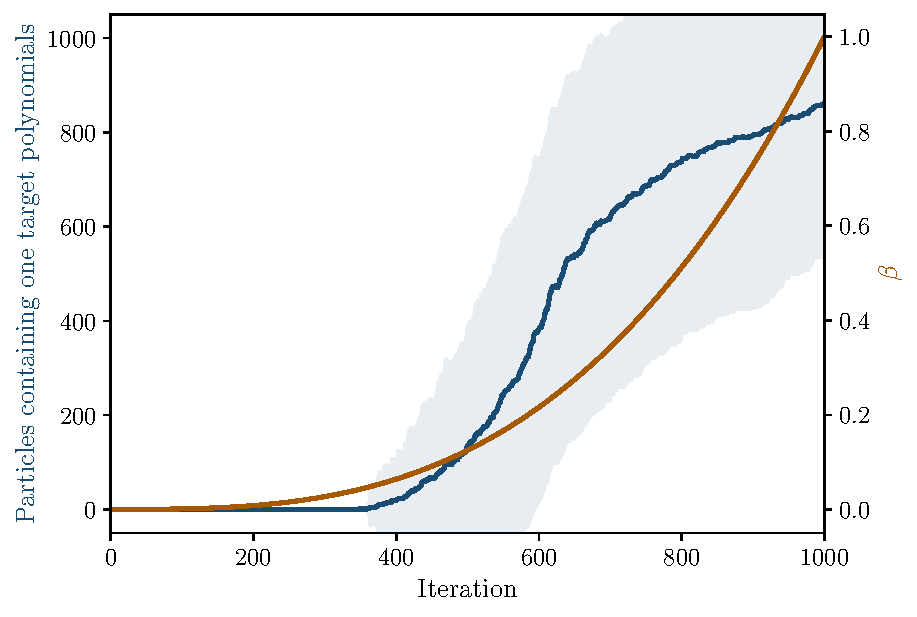
\includegraphics[scale=0.75]{Figures/Count_beta_history_2025_05_21_at_11_52_46.pdf}};
	  		\draw ($(fig1.north west) + (0,0)$) node {\small (a)};
	  		\draw (0,-8) node (fig2) {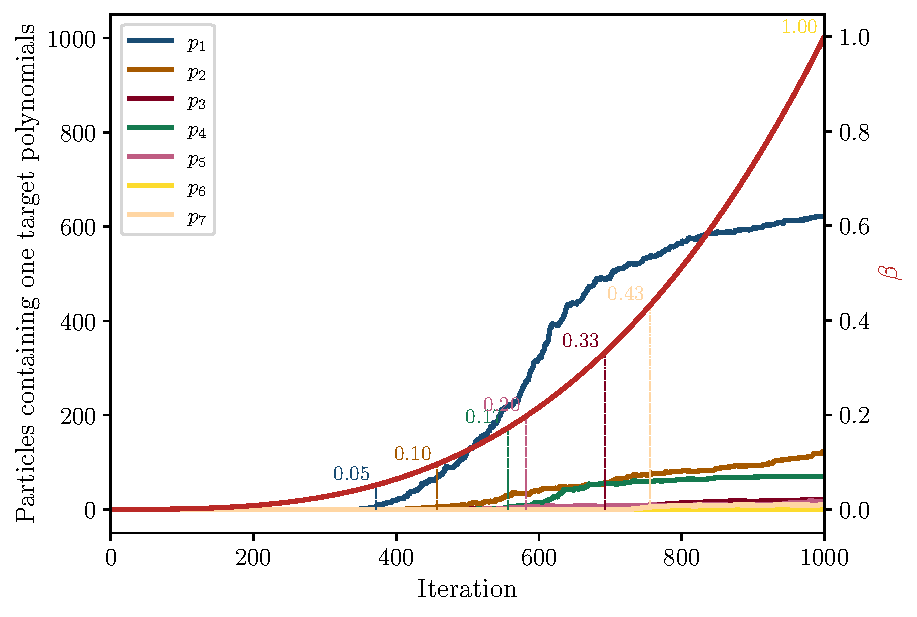
\includegraphics[scale=0.75]{Figures/Count_beta_history_2025_05_21_at_11_52_46_detailed.pdf}};
	  		\draw ($(fig2.north west) + (0,0)$) node {\small (b)};
	  	\end{tikzpicture}
	  	\caption{{\bfseries \boldmath $\beta$ in power $3$, $\sigma$ varying, $\texttt{sample size} = 10000$} (a) Evolution of the mean numbers of particles reproducing a target polynomials and its $1\sigma$ deviation for the parameters~\eqref{eq:sample10000beta3sigmavar}. (b) Evolution of the mean numbers of particles reproducing each targets polynomial. The vertical lines indicate when there are an average 5 particles reproducing a given polynomial, and the value of $\beta$ at that moment.}
	  	\label{fig:sample10000beta3sigmavar}
	  \end{figure}

	  \item {\bfseries \boldmath $\beta$ in power $5$, $\sigma=0.1$, $\texttt{sample size} = 1000$}

	  For 100 runs with parameters
		\begin{equation} \label{eq:sample1000}
			\begin{gathered}
				\texttt{max degree} = 4, \quad \texttt{max num monomials} = 6, \quad n_{\rm iter} = 1000, \quad n_{\rm particles} = 1000, \\
				\texttt{sample size} = 1000, \quad {\rm reg} = 10^{3}, \quad \beta = 10^{-10} + \left(\frac{i}{n_{\rm iter}}\right)^{5}, \quad \sigma = 0.1, \\
				p_{\rm add} = 0, \quad p_{\rm remove} = 0, \quad p_{\rm modify} = 0.5, \quad p_{\rm multiply} = 0.25, \quad p_{\rm divide} = 0.25,
			\end{gathered}
		\end{equation}
		the polynomials are found at the following frequencies
	  \begin{equation}
	  	\begin{tabular}{l|cccccccc}
	  		& $p_{1}$ & $p_{2}$ & $p_{3}$ & $p_{4}$ & $p_{5}$ & $p_{6}$ & $p_{7}$ & $\varnothing$ \\\hline\hline
	  		Frequency & 72\% & 27\% & 3\% & 19\% & 2\% & 0\% & 0\% & 12\%
	  	\end{tabular}
	  \end{equation}
	  The dynamics of the appearance of the target polynomials is plotted in fig.~\ref{fig:sample1000}.

	  Averaged number of particles reproducing a target in a successful run: $401 \pm 389$

	  Mean loss with regularisation for particles reproducing a target: $406 \pm 193$ \ce{Needs to be renormalized by the sample size.}

	  Mean loss without regularisation for particles reproducing a target: $272 \pm 192$ \ce{Needs to be renormalized by the sample size.}

	  \begin{figure}[h!]
	  	\centering
	  	\begin{tikzpicture}
	  		\draw (0,0) node (fig1) {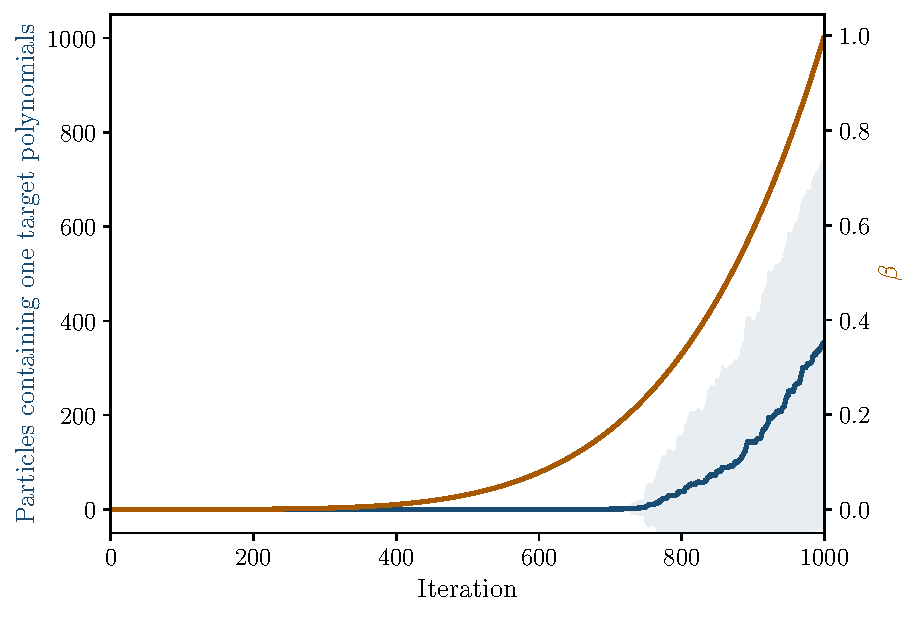
\includegraphics[scale=0.75]{Figures/Count_beta_history_2025_05_20_at_08_01_44.pdf}};
	  		\draw ($(fig1.north west) + (0,0)$) node {\small (a)};
	  		\draw (0,-8) node (fig2) {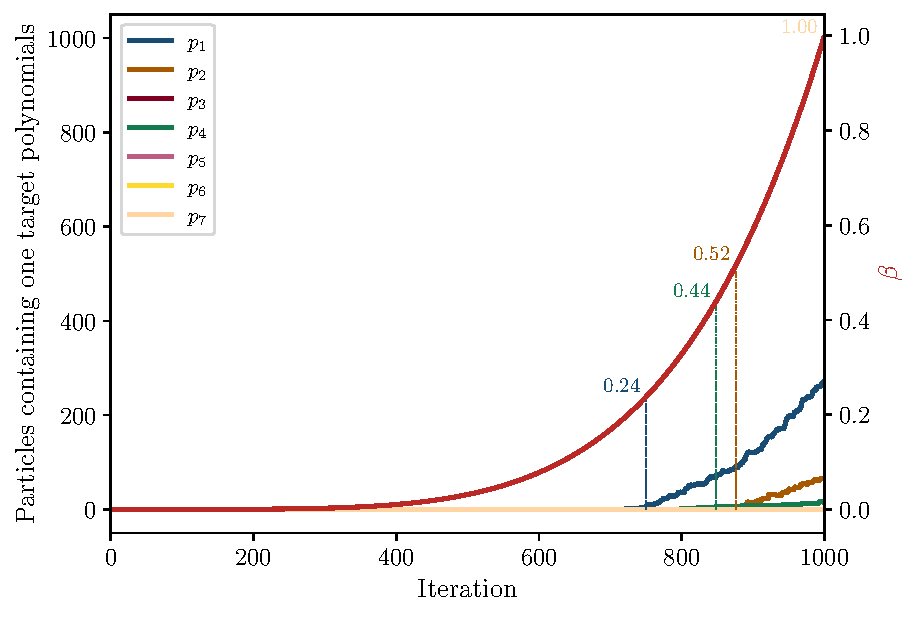
\includegraphics[scale=0.75]{Figures/Count_beta_history_2025_05_20_at_08_01_44_detailed.pdf}};
	  		\draw ($(fig2.north west) + (0,0)$) node {\small (b)};
	  	\end{tikzpicture}
	  	\caption{{\bfseries \boldmath $\beta$ in power $5$, $\sigma=0.1$, $\texttt{sample size} = 1000$} (a) Evolution of the mean numbers of particles reproducing a target polynomials and its $1\sigma$ deviation for the parameters~\eqref{eq:sample1000}. (b) Evolution of the mean numbers of particles reproducing each targets polynomial. The vertical lines indicate when there are an average 5 particles reproducing a given polynomial, and the value of $\beta$ at that moment.}
	  	\label{fig:sample1000}
	  \end{figure}
  \end{enumerate}
	

  \ce{Draw histograms of the polynomials distribution to discuss runs with multiple outputs?}

\section{Supergravity solutions}
%\begin{itemize}[label=\textbullet]
%	\item For each couple of candidate polynomials, we get the same expression for the solution, and it indeed defines a unique vacuum of the 3d SUGRA.
%	\item Discussion of the vacuum: gauge group, Zham. metric, change of variables, 3d spectrum (and stability), spin 2 spectrum on $S^{3}$, one parameter seems to be a gauge parameter, uplift?
%\end{itemize}

%For every couples $(p_{i},p_{j})$ of polynomials in eq.~\eqref{eq:pols}, the system
%\begin{equation}
%	\begin{cases}
%		p_{i} = 0, \\
%		p_{j} = 0,
%	\end{cases}
%\end{equation}
%gives the same solution \ce{That's not true! For example, $x_{1}=x_{2}=0$ solves all polynomials but is not a sugra solution. Mention tests on the sugra?}

In the previous section, we introduced a numerical method that enabled symbolic regression, yielding a set of polynomials that vanish on our dataset, as presented in Eq.~\ref{eq:pols}. We can now solve the system
\begin{equation}\label{eq:solvepol}
	p_i = 0, \quad \forall i \in {1,\dots,7}
\end{equation}
which leads to the following expressions:
\begin{equation}
	\begin{cases}
		\displaystyle x_{1} = \frac{x_{2}}{\sqrt{2}}\,\frac{e^{x_{8}/2}}{e^{x_{8}}-1}\,\Big(-x_{5}\,e^{x_{8}/2} + \sqrt{2-4\,e^{x_{8}}+e^{2x_{8}}\big(2+x_{10}^{2}\big)}\Big),\\[8pt]
		\displaystyle x_{4} = \frac{e^{-x_{8}/2}}{\sqrt{2}}\,\sqrt{2-4\,e^{x_{8}}+e^{2x_{8}}\big(2+x_{10}^{2}\big)}.
	\end{cases}
\end{equation}

Alternatively, the system can be recast as:
\begin{equation}\label{eq:rulex8x10}
	\begin{cases}
		\displaystyle \tilde{x}_{8} = \frac{x{1}^{2}+x_{2}^{2}}{x_{2}^{2} + \big(x_{1}-x_{2}x_{4}\big)^{2}},\\[10pt]
		\displaystyle x_{10} = \sqrt{2},x_{4},\frac{x_{2}^{2} - x_{1}^{2}+x_{1}x_{2}x_{4}}{x_{1}^{2}+x_{2}^{2}}.
	\end{cases}
\end{equation}

As anticipated, this defines a three-parameter solution corresponding to a three-dimensional slice of the half-maximal supergravity scalar potential.

Let us make a few remarks at this stage. First, it is possible to find solutions to Eq.~\ref{eq:solvepol} which, however, are not solutions of $\nabla V = 0$. For instance $x_1 = x_2 = 0$; such cases are excluded, as they do not satisfy the stationarity condition and therefore do not correspond to valid physical solutions.

Secondly, one might argue that only two of the seven polynomials are sufficient to fully characterize the solution. That is, choosing any pair $(i,j) \in {1, \dots, 7}$ may suffice to extract a complete description. In practice, this is not entirely accurate. While such a pair can yield partial constraints—for example, recovering Eq.\ref{eq:rulex8x10}—it may also produce alternative (and potentially less general) parameterizations. Upon inspection, all such partial rules are found to be consistent with, and included in, the most general expressions given in Eq.\ref{eq:rulex8x10}.

The solution preserves a ${\rm U}(1)\times{\rm U}(1)$ gauged symmetry.

%\paragraph{Moduli space}
The $(x_{1},x_{2},x_{4})$ moduli space is most nicely parametrised using the change of coordinates
\begin{equation}
	x_{1} = r\cos(\theta)\cos(\Phi), \quad x_{2} = r\cos(\theta)\sin(\Phi) \quad {\rm and} \quad x_{4} = r\sin(\theta),
\end{equation}
for which the Zamolodchikov metric reads
\begin{equation}
	\d^{2}s_{\rm Zam.} = -\,\d r^{2} - r^{2}\,\bigg(\d \theta^{2} - r\cos(\theta)\,\d \theta\d\Phi + \sin(\theta)\,\d r\d\Phi + \frac{1}{2}\,\big(3+r^{2}-\cos(2\theta)\big)\,\d\Phi^{2} \bigg).
\end{equation}
\ce{Tests other change of variables? Test choices of variables other than $(x_{1},x_{2},x_{4})$?}

\paragraph{Bosonic spectrum}
Vector fields:
\begin{equation}
 \begin{aligned}	
	m_{\sst{(1)}}\ell_{\rm AdS}:\quad &
	0\ [2],	\quad
	-2\ [5],	\quad
	2\ [1],	\\[5pt]
	&	-1\pm\sqrt{\left(1+r^2\right)^2-2\,r^2\,\cos(2\theta)}\ [2+2],	\\[5pt]
	&	1\pm\sqrt{1+4\,r^2+r^{4}}\ [2+2].
 \end{aligned}
\end{equation}
The integers between square brackets indicate the multiplicity of each eigenvalue. The spectrum includes two massless vectors corresponding to the unbroken ${\rm U}(1)\times {\rm U}(1)$ gauge symmetry, although in three dimensions they are non-propagating.


Scalars:
\begin{equation}
 \begin{aligned}	
	\left(m_{\sst{(0)}}\ell_{\rm AdS}\right)^2:\quad&
	0\ [5],	\quad
	8\ [1],	\quad
	r^{2}\,\left(4+r^2\right)\ [8],	\\[5pt]
	&	2r\,\Big(3\,r+r^{3}\pm(2+r^{2})\,\sqrt{2+r^2-2\,\cos(2\theta)}-r\cos(2\theta)\Big)\ [2+2].
 \end{aligned}
\end{equation}

Gravitini:
\begin{equation}
	m_{{(\nicefrac32)}}\ell_{\rm AdS}:\quad 
	\quad \dfrac1{2}\bigg[1\pm\sqrt{4+2\,r^{2}+r^{4}-2r^{2}\cos(2\theta)}\bigg]\ [4+4],
\end{equation}
no SUSY enhancements other than $r=0$.

No dependence on $\Phi$.

\section{Conclusion}
\begin{itemize}[label=\textbullet]
	\item Conclusion: good prospects of improvement to be able to access higher dimensional cases. Classify flat directions.
	\item Appendix with some details on the code?

\end{itemize}

In this work, we have presented a novel machine learning approach to systematically identify and characterize flat directions in supergravity scalar potentials. Our methodology combines gradient descent sampling with annealed importance sampling for symbolic regression, demonstrating its effectiveness on a 5-scalar subsector of 3d (2,0) supergravity derived from 
$AdS_3 \times S^3 \times T^4$ compactifications of IIB supergravity.

We developed a robust pipeline that transitions from numerical exploration to analytical understanding. The gradient descent procedure successfully samples the flat direction manifold, while local PCA analysis reveals its intrinsic dimensionality. Most notably, our annealed importance sampling approach to symbolic regression automatically discovers polynomial constraints characterizing the manifold, bypassing the computational complexity that renders direct symbolic manipulation intractable.

Our analysis reveals that the 5-dimensional scalar space contains a 3-dimensional conformal manifold, with one direction potentially gauge-fixable. The discovered solution preserves $U(1) \times U(1)$ gauged symmetry and exhibits a rich spectrum structure. The Zamolodchikov metric on the moduli space, parametrized by spherical-like coordinates, provides a concrete geometric description of the conformal manifold.

The method demonstrates remarkable efficiency and reliability. Across different parameter choices, we achieve success rates of 69-76\% for the most common polynomial constraint, with computation times of approximately 700 seconds per run on standard hardware. The algorithm discovers seven distinct polynomial relations with varying frequencies, suggesting a hierarchical structure in constraint discovery.

This approach opens several promising avenues for advancement. The scalability to higher-dimensional cases represents the most immediate challenge and opportunity. By increasing the number of particles, refining the annealing schedule, and optimizing polynomial search strategies, we anticipate extending this methodology to the full 13-scalar theory and potentially to other supergravity models.

Beyond technical improvements, this work suggests a broader paradigm for studying conformal manifolds in string theory and supergravity. The ability to automatically extract analytical constraints from numerical data could prove invaluable for classifying flat directions across different theories, understanding moduli stabilization mechanisms, and exploring the landscape of consistent supergravity backgrounds.

The marriage of machine learning techniques with traditional supergravity analysis represents a step toward more systematic approaches to understanding the rich geometric structures underlying these theories. As computational power increases and algorithms improve, we envision this methodology becoming a standard tool for exploring the intricate relationships between geometry, symmetry, and dynamics in supergravity theories.

While the specific solution found in this 5-scalar model may have limited direct physical applications, the demonstrated feasibility of our approach and its potential for systematic classification of flat directions across the supergravity landscape make it a valuable addition to the theoretical physicist's toolkit.

\bibliography{references}


\end{document}
